\documentclass[11pt]{article}

\usepackage[margin=1in]{geometry}
\usepackage{amsmath,amssymb}
\usepackage{graphicx}
\usepackage{booktabs}
\usepackage[colorlinks=true,linkcolor=blue,citecolor=blue,urlcolor=blue]{hyperref}
\usepackage{natbib}

\graphicspath{{../figures/}}

% \code tokens (tags, filenames, test names) carry no discretionary
% breaks, so a paragraph containing one can have no acceptable line
% break at all.  emergencystretch gives TeX the slack to set those
% lines loose rather than overfull.
\setlength{\emergencystretch}{3em}

\newcommand{\rmu}{\ensuremath{\mathrm{rad\,m^{-2}}}}
\newcommand{\lamsq}{\ensuremath{\lambda^{2}}}
\newcommand{\code}[1]{\texttt{#1}}

% EVERY number in this document comes from here, and generated.tex is
% written by scripts/step5_tables.py straight from the npz products.
% Do not type a number into this file.  Two published errors -- the
% tail gate's inconsistent threshold and the closed-form "within a few
% percent" claim -- were hand-transcription drifting from the products
% it claimed to summarise.
% GENERATED by scripts/step5_tables.py -- do not edit.
% Regenerate:  uv run python scripts/step5_tables.py
\newcommand{\Lunations}{24}
\newcommand{\SafeCut}{27.5}
\newcommand{\detNoCutSlabThirty}{32.1}
\newcommand{\detNoCutDispThirty}{0.039}
\newcommand{\detSafeSlabThirty}{13.6}
\newcommand{\detSafeDispThirty}{0.017}
\newcommand{\keepFracThirty}{27}
\newcommand{\cutCostThirty}{2.4}
\newcommand{\tauSafeThirty}{58.3}
\newcommand{\amfNoCutThirty}{\ensuremath{1.33\times10^{-5}}}
\newcommand{\amfSafeThirty}{\ensuremath{1.63\times10^{-5}}}
\newcommand{\tailSlabThirty}{1.63}
\newcommand{\tailSlabTwoPortThirty}{1.62}
\newcommand{\tailFracThirty}{0.47}
\newcommand{\dispGapNoCutThirty}{25.4}
\newcommand{\dispTimeNoCutThirty}{647}
\newcommand{\dispGapSafeThirty}{60.3}
\newcommand{\dispTimeSafeThirty}{3632}
\newcommand{\detNoCutSlabFifty}{109.0}
\newcommand{\detNoCutDispFifty}{0.376}
\newcommand{\detSafeSlabFifty}{52.4}
\newcommand{\detSafeDispFifty}{0.181}
\newcommand{\keepFracFifty}{27}
\newcommand{\cutCostFifty}{2.1}
\newcommand{\tauSafeFifty}{12.6}
\newcommand{\amfNoCutFifty}{\ensuremath{1.07\times10^{-5}}}
\newcommand{\amfSafeFifty}{\ensuremath{1.16\times10^{-5}}}
\newcommand{\tailSlabFifty}{6.84}
\newcommand{\tailSlabTwoPortFifty}{7.64}
\newcommand{\tailFracFifty}{0.65}
\newcommand{\dispGapNoCutFifty}{2.7}
\newcommand{\dispTimeNoCutFifty}{7}
\newcommand{\dispGapSafeFifty}{5.5}
\newcommand{\dispTimeSafeFifty}{31}
\newcommand{\detNoCutSlabTen}{3.0}
\newcommand{\detNoCutDispTen}{\ensuremath{3.9\times10^{-4}}}
\newcommand{\detSafeSlabTen}{1.3}
\newcommand{\detSafeDispTen}{\ensuremath{1.7\times10^{-4}}}
\newcommand{\keepFracTen}{26}
\newcommand{\cutCostTen}{2.2}
\newcommand{\tauSafeTen}{1573.5}
\newcommand{\amfNoCutTen}{\ensuremath{1.67\times10^{-5}}}
\newcommand{\amfSafeTen}{\ensuremath{1.92\times10^{-5}}}
\newcommand{\tailSlabTen}{0.17}
\newcommand{\tailSlabTwoPortTen}{0.17}
\newcommand{\tailFracTen}{0.54}
\newcommand{\dispGapNoCutTen}{2595.7}
\newcommand{\dispTimeNoCutTen}{\ensuremath{6.7\times10^{6}}}
\newcommand{\dispGapSafeTen}{5827.8}
\newcommand{\dispTimeSafeTen}{\ensuremath{3.4\times10^{7}}}
\newcommand{\DetectionRows}{%
no cut & 100\% & 32.1 & 0.039 & 109.0 & 0.376 & 3.0 & \ensuremath{3.9\times10^{-4}} \\
$\geq 5$ & 66\% & 25.6 & 0.031 & 85.9 & 0.296 & 2.4 & \ensuremath{3.1\times10^{-4}} \\
$\geq 10$ & 50\% & 20.5 & 0.025 & 73.9 & 0.255 & 2.1 & \ensuremath{2.7\times10^{-4}} \\
$\geq 27.5$ & 27\% & 13.6 & 0.017 & 52.4 & 0.181 & 1.3 & \ensuremath{1.7\times10^{-4}} \\
$\geq 50$ & 17\% & 9.8 & 0.012 & 35.7 & 0.123 & 1.0 & \ensuremath{1.3\times10^{-4}} \\
$\geq 100$ & 9\% & 7.0 & 0.009 & 24.1 & 0.083 & 0.7 & \ensuremath{9.0\times10^{-5}} \\
$\geq 200$ & 4\% & 4.8 & 0.006 & 15.5 & 0.054 & 0.5 & \ensuremath{5.9\times10^{-5}} \\
$\geq 400$ & 1\% & 3.0 & 0.004 & 8.9 & 0.031 & 0.3 & \ensuremath{3.4\times10^{-5}} \\
}
\newcommand{\bracketUpperThirty}{\ensuremath{9.89\times10^{-3}}}
\newcommand{\bracketUpperFifty}{\ensuremath{8.98\times10^{-3}}}
\newcommand{\bracketUpperTen}{\ensuremath{1.08\times10^{-2}}}
\newcommand{\bracketSlabThirty}{\ensuremath{4.27\times10^{-4}}}
\newcommand{\bracketSlabFifty}{\ensuremath{1.17\times10^{-3}}}
\newcommand{\bracketSlabTen}{\ensuremath{4.95\times10^{-5}}}
\newcommand{\bracketDispThirty}{\ensuremath{5.22\times10^{-7}}}
\newcommand{\bracketDispFifty}{\ensuremath{4.03\times10^{-6}}}
\newcommand{\bracketDispTen}{\ensuremath{6.45\times10^{-9}}}
\newcommand{\BracketRows}{%
$A_{\rm upper}$ & \ensuremath{9.89\times10^{-3}} & \ensuremath{8.98\times10^{-3}} & \ensuremath{1.08\times10^{-2}} \\
$A_{\rm slab}$ & \ensuremath{4.27\times10^{-4}} & \ensuremath{1.17\times10^{-3}} & \ensuremath{4.95\times10^{-5}} \\
$A_{\rm disp}$ & \ensuremath{5.22\times10^{-7}} & \ensuremath{4.03\times10^{-6}} & \ensuremath{6.45\times10^{-9}} \\
}
\newcommand{\resAmpThirty}{7.592}
\newcommand{\resPowThirty}{5.574}
\newcommand{\cutResThirty}{3.6}
\newcommand{\resAmpFifty}{35.150}
\newcommand{\resPowFifty}{25.805}
\newcommand{\cutResFifty}{0.8}
\newcommand{\resAmpTen}{0.281}
\newcommand{\resPowTen}{0.206}
\newcommand{\cutResTen}{97.8}
\newcommand{\ResolutionRows}{%
30\,MHz & 5.574 & \textbf{7.592} & 7.632 \\
50\,MHz & 25.805 & \textbf{35.150} & 35.334 \\
10\,MHz & 0.206 & \textbf{0.281} & 0.283 \\
}
\newcommand{\parentHorFifty}{58.03}
\newcommand{\zoomHorFifty}{2796.9}
\newcommand{\parentHorThirty}{12.54}
\newcommand{\zoomHorThirty}{604.1}
\newcommand{\parentHorTen}{0.46}
\newcommand{\zoomHorTen}{22.4}
\newcommand{\HorizonRows}{%
50\,MHz & 58.03 & 2796.9 \\
30\,MHz & 12.54 & 604.1 \\
10\,MHz & 0.46 & 22.4 \\
}
\newcommand{\pFifty}{23.4}
\newcommand{\pNinety}{185.7}
\newcommand{\pNineNine}{776.1}
\newcommand{\pNineNineNine}{1283.0}
\newcommand{\rmMax}{2442.1}
\newcommand{\kneeThirty}{89.6}
\newcommand{\taperFactorThirty}{4.99}
\newcommand{\armSwapThirty}{-0.7}
\newcommand{\kneeFifty}{83.3}
\newcommand{\taperFactorFifty}{4.33}
\newcommand{\armSwapFifty}{+23.6}
\newcommand{\kneeTen}{83.9}
\newcommand{\taperFactorTen}{4.66}
\newcommand{\armSwapTen}{+12.1}
\newcommand{\RobustnessRows}{%
30\,MHz & 89.62 & 17.95 & 4.99$\times$ & 88.99 & -0.7\% \\
50\,MHz & 83.32 & 19.26 & 4.33$\times$ & 102.99 & +23.6\% \\
10\,MHz & 83.91 & 18.03 & 4.66$\times$ & 94.09 & +12.1\% \\
}
\newcommand{\chirpPctThirty}{2.0}
\newcommand{\aliasPctThirty}{1.8}
\newcommand{\aliasWallThirty}{604}
\newcommand{\zoomHorFromNyqThirty}{604.0}
\newcommand{\chirpPctFifty}{1.2}
\newcommand{\aliasPctFifty}{0.0}
\newcommand{\aliasWallFifty}{2796}
\newcommand{\zoomHorFromNyqFifty}{2796.4}
\newcommand{\chirpPctTen}{6.0}
\newcommand{\aliasPctTen}{115.1}
\newcommand{\aliasWallTen}{22}
\newcommand{\zoomHorFromNyqTen}{22.4}
\newcommand{\BasisRows}{%
30\,MHz & 386 & 7.7 & \textbf{2.0\%} & 604 & 1.8\% \\
50\,MHz & 83 & 1.0 & \textbf{1.2\%} & 2796 & 0.0\% \\
10\,MHz & 10425 & 625.5 & \textbf{6.0\%} & 22 & 115.1\% \\
}
\newcommand{\thetaCDeg}{0.2}
\newcommand{\thetaCAllClamped}{yes}
\newcommand{\tsysThirty}{1.0044}
\newcommand{\tsysFifty}{1.0170}
\newcommand{\tsysTen}{1.0006}
\newcommand{\tsysMaxPct}{1.7}


\title{Detecting Galactic Faraday rotation with LuSEE-Night:\\
  sensitivity, systematics separation, and the depolarisation floor}
\author{Christian Hellum Bye}
\date{2026-08-21}

\begin{document}
\maketitle

\begin{abstract}
\noindent
LuSEE-Night observes the polarized synchrotron sky through the Galactic
Faraday screen at 10--50\,MHz. This report asks whether the instrument
can \emph{detect} Faraday rotation at all --- not whether it can
resolve the Galactic rotation-measure distribution, which it cannot ---
and what limits that detection.

The central methodological result is an estimator. The earlier diffuse
calculation summed the Faraday phasor pixel by pixel over a HEALPix
map; that is a random walk whose amplitude falls as
$N_{\rm pix}^{-1/2}$, so it was measuring pixelisation shot noise
rather than sky. Binning the beam- and emissivity-weighted sky
\emph{in Faraday depth first} and transforming second gives a
distribution $F(\phi)$ whose shape is invariant under refinement, and
whose dependence on the one free input --- where synchrotron emission
sits along the rotating column --- moves the detection number by a
factor \kscanAmpThirty{} rather than by an order of magnitude. (The same
distribution can be read out in delay rather than depth with no loss;
Appendix~\ref{sec:bases} shows why, since the superseded analysis
worked there.)

The detection result is a curve, not a number, because the useful
statistic must discard the low-depth region where spectrally smooth
$I\!\to\!Q,U$ leakage lives. Cutting at $\phi \ge \SafeCut$\,\rmu, where
window leakage falls below $10^{-6}$ of Stokes $I$, retains
$\keepFracThirty$\% of the template power and costs only a factor
$\cutCostThirty$ in sensitivity. After that cut, a diffuse amplitude at
the uniform-slab depolarisation floor is detectable at
$\detSafeSlabThirty\times$ threshold at 30\,MHz and
$\detSafeSlabFifty\times$ at 50\,MHz in \Lunations{} lunations; at the
internal-dispersion floor it is undetectable at every band, with
50\,MHz closest at $\detSafeDispFifty$.

The science case therefore turns on a single unknown --- which
depolarisation floor the interstellar medium sets, a
mixed-versus-external-screen geometry question --- and not on the
instrument, the emissivity geometry, the analysis basis, or the
integration time.
\end{abstract}

\tableofcontents

\section{What is being asked}
\label{sec:scope}

\subsection{Detection, not localisation}

These are different questions with different statistics and very
different answers, and conflating them is the main way to misread this
subject.

\emph{Localisation} asks whether a feature can be placed on the Faraday
depth axis and mapped to Galactic structure. That needs resolution,
deconvolution, and signal power in a region distinguishable from the
bulk of the sky's depth distribution. Section~\ref{sec:tail} shows it is
marginal at best.

\emph{Detection} asks whether there is any evidence of Faraday rotation
that cannot be explained by an instrumental systematic. That needs SNR
and a statistic that is not degenerate with the systematics. It is a
far weaker requirement, and it is what this report is about.

An earlier version of this document led with the localisation verdict
and quoted its integration cost --- tens of thousands of nights --- as
though it were the detection answer. It is not: after the systematics
cut, the detection gap at the internal-dispersion floor at 50\,MHz is
$\dispGapSafeFifty\times$, an observing-time factor of
$\dispTimeSafeFifty$, not $10^4$.

\subsection{What is predicted, and what is not}

This report predicts a normalised \emph{shape} in Faraday depth and a
detectability threshold against it. It does not predict the amplitude
of the diffuse Faraday signal; that is quoted as a bracket with
reasons, and Section~\ref{sec:cannot} shows exactly where the amplitude
calculation runs out of information.

Three things are inputs, not results, and are owned elsewhere: the
instrument response and covariance assembly (\code{luseepy}), the
spherical transforms and polarized harmonic dual (\code{croissant}),
and the Galactic Faraday depth map \citep{hutschenreuter2022}. This
work owns the layer above.

\subsection{Relation to the earlier analysis}
\label{sec:supersede}

An earlier four-port analysis, together with the numerical audit that
refuted part of it, is preserved at the repository tag
\code{audit-2026-08-18}. Section~\ref{sec:reconcile} gives the
section-by-section status; the short form is that Steps 0, 1 and 3 and
the $I$-only limit stand, and Steps 2 and 4 are refuted by
Section~\ref{sec:randomwalk}.

\section{Faraday rotation in the harmonic dual}
\label{sec:dual}

For a linearly polarized sky, propagation through a magnetised plasma
of Faraday depth $\phi$ rotates the polarization vector. In the
\code{healpy}/COSMO convention used for all input maps,
\begin{equation}
  (Q + iU)_{\rm COSMO} \;\longrightarrow\; (Q + iU)_{\rm COSMO}\,
  e^{+2i\phi\lamsq},
  \label{eq:faraday}
\end{equation}
with $\lamsq = (c/\nu)^2$ in $\mathrm{m^2}$ and $\phi$ in \rmu. The
factor of two is the spin weight of linear polarization.
Spherical-harmonic machinery consumes the IAU convention, in which
$U_{\rm IAU} = -U_{\rm COSMO}$, so $(Q+iU)_{\rm IAU} =
\overline{(Q+iU)_{\rm COSMO}}$ for real maps.

The polarized harmonic dual holds spin-$\pm2$ blocks $P_{-}$ (the spin
$-2$ analysis of $(Q+iU)_{\rm IAU}$) and $P_{+}$, alongside spin-0 $I$
and $V$. Combining the two conventions, Faraday rotation acts as
\begin{equation}
  \bigl(I,\;V,\;P_{-},\;P_{+}\bigr) \;\longrightarrow\;
  \bigl(I,\;V,\;e^{-2i\phi\lamsq}P_{-},\;e^{+2i\phi\lamsq}P_{+}\bigr).
  \label{eq:dualblock}
\end{equation}

Equation~\eqref{eq:dualblock} is the structural fact the calculation
rests on: \textbf{Faraday rotation is diagonal in the harmonic dual}.
It multiplies each block by a scalar depending on frequency and depth
but not on $\ell$ or $m$, so a region of constant depth needs one
frequency-independent set of $a_{\ell m}$ plus per-frequency scalars.
That is what makes a 16\,384-channel fine grid affordable: the
expensive contraction of sky against response harmonics is done once
per component, and frequency dependence is applied afterwards.

\section{The four-port response and the Faraday weight}
\label{sec:weight}

The instrument is a four-port system, ports $\mathrm{N,E,S,W}=0,1,2,3$,
read out as sixteen real cross-power channels. Each port pair responds
to the sky through a pair-Stokes kernel $(K_I,K_Q,K_U,K_V)(\hat n)$.

A Faraday-rotated sky enters through $K_Q$ and $K_U$ only:
\begin{equation}
  K_Q Q + K_U U =
  \Re\Bigl[(K_Q - iK_U)\,(Q+iU)\,e^{2i\phi\lamsq}\Bigr].
\end{equation}
The intrinsic polarization angle is unknown and effectively random from
direction to direction, so what survives is the
\emph{basis-independent} combination
\begin{equation}
  |w(\hat n)| = \sqrt{\tfrac12\bigl(|K_Q(\hat n)|^2 + |K_U(\hat
  n)|^2\bigr)},
  \label{eq:weight}
\end{equation}
averaged over pairs and over local sidereal time. Using $|K_Q|$ alone
would make every percentile and template below depend on the arbitrary
orientation of the $Q/U$ basis.

Figure~\ref{fig:weight} shows $|w|^2$. The Galactic plane dominates ---
which is why the plane taper of Section~\ref{sec:robust} moves the
roll-off so far --- and a contiguous cap carries exactly zero weight,
being never above the horizon at the landing site.

\begin{figure}[htbp]
  \centering
  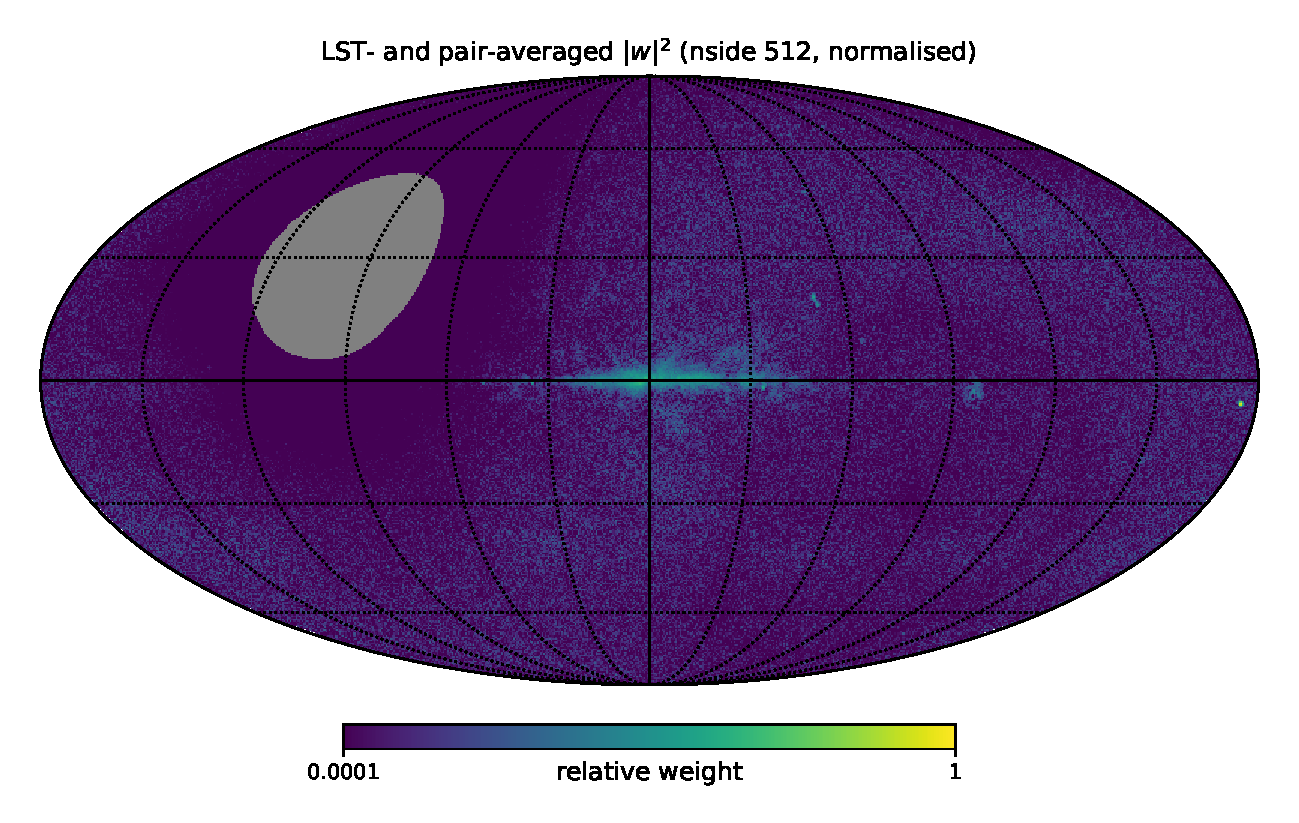
\includegraphics[width=0.72\textwidth]{step5_weight_map.pdf}
  \caption{The LST- and pair-averaged Faraday weight $|w|^2$,
  Equation~\eqref{eq:weight}, at nside 512 in Galactic coordinates,
  normalised and logarithmic. Grey: sky never above the horizon, which
  carries exactly zero weight. Every sky percentile in this report is
  weighted by this map.}
  \label{fig:weight}
\end{figure}

Because the beam enters only through $|w|^2$, swapping the as-built
four-port response for the symmetric two-port pseudo-dipole is one
input substitution, which makes the arm comparison in
Section~\ref{sec:robust} a genuine robustness test.

\section{Why the pixel-space sum fails}
\label{sec:randomwalk}

The earlier calculation formed the observable as a coherent pixel sum,
\begin{equation}
  P(\lamsq) = \sum_{n} w_n\, e^{2i\phi_n \lamsq},
  \label{eq:pixelsum}
\end{equation}
and read an amplitude off it. That estimator does not converge to a sky
quantity.

Write $w_n = |w_n|e^{i\alpha_n}$ and $\theta_n = \alpha_n +
2\phi_n\lamsq$. The intrinsic angles $\alpha_n$ are effectively random
between pixels, and so is $2\phi_n\lamsq$ modulo $2\pi$. The Faraday
map is a smooth reconstruction, so neighbouring nside-512 pixels are
not far apart in depth --- a median $\adjMedian$\,\rmu, a p90 of
$\adjPninety$ --- but at these wavelengths that is already many turns
of the carrier: $\adjTurnsThirty$ between a median neighbour pair at
30\,MHz, $\adjTurnsTen$ at 10\,MHz and $\adjTurnsFifty$ at 50\,MHz.
Then
\begin{equation}
  \bigl\langle |P|^2 \bigr\rangle
  = \sum_{n,m} |w_n||w_m|\bigl\langle e^{i(\theta_n-\theta_m)}\bigr\rangle
  = \sum_{n} |w_n|^2 ,
  \label{eq:walk}
\end{equation}
every cross term averaging to zero, and for $N$ pixels of comparable
weight the \emph{normalised} amplitude behaves as
\begin{equation}
  \frac{\sqrt{\langle |P|^2\rangle}}{\sum_n |w_n|}
  = \frac{\sqrt{N}|w|}{N|w|} = N^{-1/2}.
  \label{eq:nhalf}
\end{equation}

Equation~\eqref{eq:nhalf} is a statement about the estimator, not the
sky: its value is set by how finely the sphere is pixelised and it goes
to zero under refinement. The direct demonstration is the acceptance
gate of Section~\ref{sec:gates}, where nside $256 \to 2048$ collapses
the coherent power by a factor $134$ --- close to the factor $64$
Equation~\eqref{eq:nhalf} predicts, and nothing like the invariance a
physical signal would show.

The sum in Equation~\eqref{eq:pixelsum} is computed correctly, and it
is not wrong in general --- it is the standard RM-synthesis estimator,
and it is the right one at the frequencies where the Faraday map itself
was measured. Coherence across a pixel needs
$2\,\Delta\mathrm{RM}\,\lamsq \lesssim 1$, which for the median
neighbour pair holds above $\sim\cohValidMHz$\,MHz. \textbf{LuSEE-Night
observes about a decade below that floor}, which is the whole of the
difference: the same estimator that builds the input map cannot be used
on the data the map is being applied to.

Figure~\ref{fig:bridge} makes that quantitative by scaling the RM map
down until the estimator does converge. It converges where the sky is
weak enough that the Faraday phase varies slowly between neighbouring
pixels --- and \emph{that regime has no signal to measure}, because the
whole depth distribution then sits at $\phi\approx0$, inside the region
Section~\ref{sec:detection} must discard as degenerate with smooth
leakage. The two regimes are disjoint. That is why the estimator had to
be replaced rather than repaired.

\begin{figure}[htbp]
  \centering
  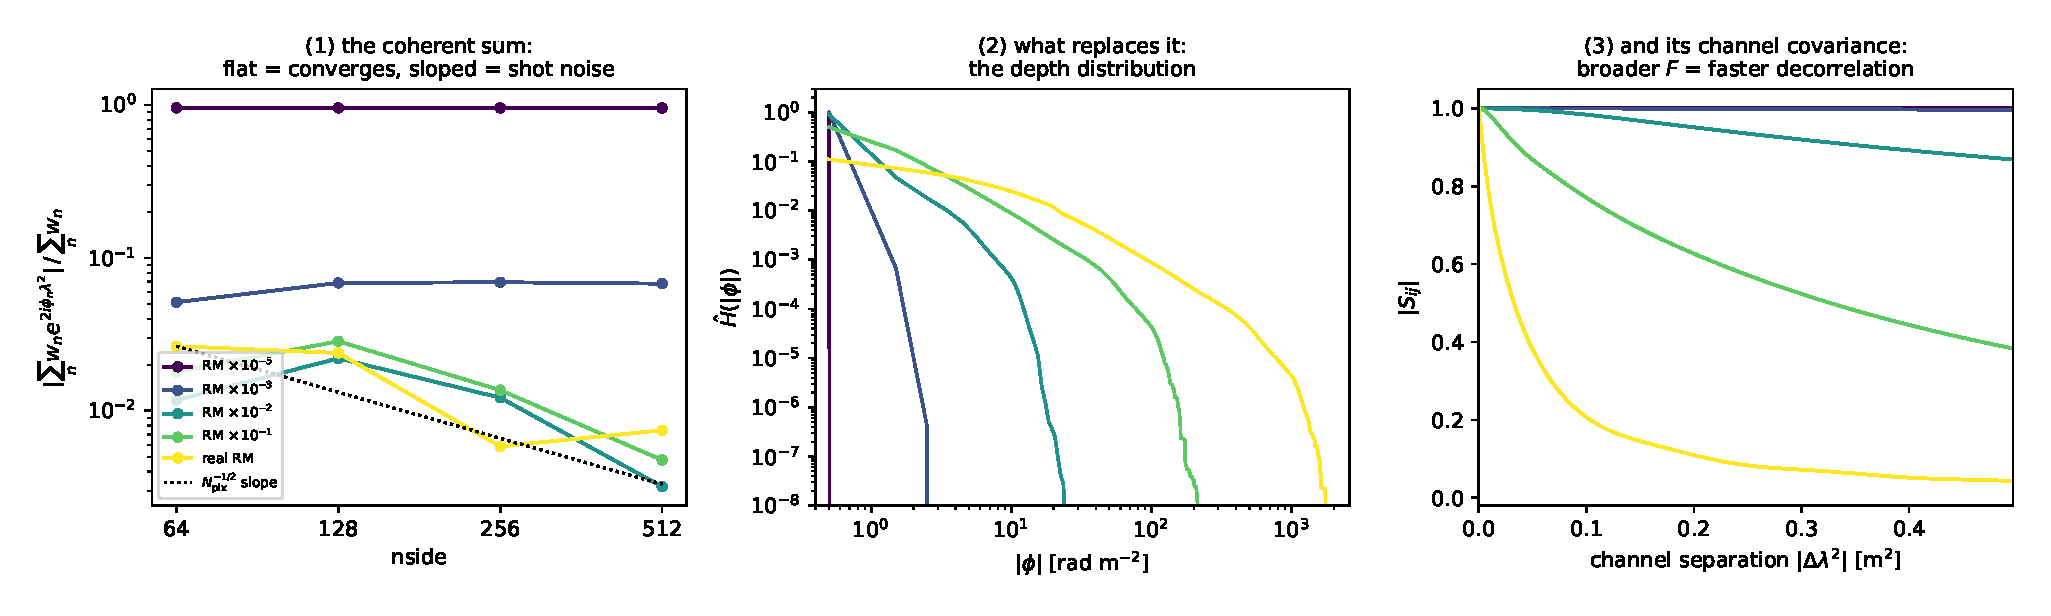
\includegraphics[width=\textwidth]{step5_bridge.pdf}
  \caption{Scaling the Galactic RM map down moves it from the regime
  where the coherent pixel sum converges to the regime where it is a
  random walk. Left: the estimator against pixelisation --- flat means
  it converges, sloped means it is measuring $N_{\rm pix}$. Intrinsic
  angles are set to zero (maximally coherent), so any decay is the
  Faraday phase decorrelating and not the sky's angles. Middle and
  right: the depth distribution that replaces it, and the channel
  covariance that follows. Reading one colour left to right is one
  sky.}
  \label{fig:bridge}
\end{figure}

\section{The depth distribution and its transform}
\label{sec:depthdist}

\subsection{Why the power estimator is the right target}
\label{sec:identity}

Substituting Equation~\eqref{eq:pixelsum} into the depth transform and
expanding,
\begin{equation}
  \bigl\langle |\tilde P(\phi)|^2 \bigr\rangle
  = \sum_{n} |w_n|^2 \bigl|R(\phi-\phi_n)\bigr|^2
  + \underbrace{\sum_{n \ne m} |w_n||w_m|
    \bigl\langle e^{i(\alpha_n-\alpha_m)}\bigr\rangle
    R(\phi-\phi_n)\overline{R(\phi-\phi_m)}}_{\to\,0},
  \label{eq:identity}
\end{equation}
with $R$ the point-spread function of Section~\ref{sec:rmsf}. The first
term is $F$ convolved with $|R|^2$. \textbf{The same sum that fails as
an \emph{amplitude} estimator succeeds as a \emph{power} estimator}:
the shot noise of Equation~\eqref{eq:walk} is precisely the diagonal
term Equation~\eqref{eq:identity} wants. That is the licence for
everything below --- the object worth predicting is a distribution of
polarized \emph{power} over depth, and the rest of this section
constructs it.

Measured with real WMAP K-band polarization angles \citep{bennett2013}
supplying $\alpha_n$, the ratio of the two sides is $1.069$ over
$30 \le |\phi| < 1500$\,\rmu{} at 30\,MHz, and $1.332$ over the whole
axis; the difference is the $|\phi|<10$ region where the pixel sum is
genuinely partly coherent. Read this as an \emph{independent
confirmation that the ratio is consistent with unity}, not as
reproducing a particular number: the audit's comparable figure of
$1.038$ used a different window, grid and estimator, and is one of a
series running $1.010/1.184/1.038/0.843$ across nside.

It is a test, not an identity --- falsification probes break it ($k=0$
against a $k\to\infty$ observable gives $1.85$, a shuffled RM map
$1.58$, and the $\mathrm{RM}\times0.02$ control fails by $>10^4$). But
two limits are worth stating. It does \emph{not} show the sky is
incoherent: with $\alpha_n \equiv 0$, maximally coherent, it still
passes at $0.889$, because one carrier turn is a depth separation of
$\pi/\lamsq = 0.0315$\,\rmu{} at 30\,MHz and the cross terms cancel by
oscillation rather than by phase randomness. Nor does it pass only on
WMAP K noise: smoothing $Q,U$ to $3^\circ$ and $10^\circ$ gives
$1.107$ and $1.143$.

\subsection{Bin first, transform second}

Reverse the order of operations. Accumulate $|w_n|^2$ into depth bins
to form $F(\phi)$, then transform:
\begin{equation}
  P(\lamsq) = \int F(\phi)\, e^{2i\phi\lamsq}\,\mathrm d\phi .
  \label{eq:rmsynth}
\end{equation}
Equation~\eqref{eq:rmsynth} is the standard RM-synthesis relation
\citep{burn1966,brentjens2005}. What changes is the order.

Concretely, the accumulation is a \emph{weighted histogram}: the RM map
supplies each pixel's bin \textbf{index} and the beam-sky weight
supplies the \textbf{mass} deposited there. Writing $w_n(t)$ for
Equation~\eqref{eq:weight} at pixel $n$ and local sidereal time $t$,
multiplied by the polarized emissivity of that pixel and summed in
quadrature over port pairs, each pixel deposits its whole weight in
the one bin $b = [\phi_b, \phi_{b+1})$ containing its column depth:
\begin{equation}
  F_b^{(\infty)} \;=\; \sum_{t}\sum_{n} w_n(t)^2 \,
  \mathbf{1}\!\left[\phi_{{\rm col},n} \in b\right] .
  \label{eq:histogram}
\end{equation}
That is the blue curve of Figures~\ref{fig:inputs}
and~\ref{fig:family}. The two maps enter at native nside 512 with
one-to-one pixel correspondence, and the weight is recomputed at every
$t$ because the beam moves over the sky.

Equation~\eqref{eq:histogram} assumes all the emission sits behind all
the rotation. It does not, and Section~\ref{sec:pushforward} replaces
the indicator by an emissivity kernel $C_n$ that spreads each pixel's
weight along its own column,
\begin{equation}
  F_b \;=\; \sum_{t}\sum_{n} w_n(t)^2 \,
  \bigl[\,C_n(\phi_{b+1}) - C_n(\phi_b)\,\bigr],
  \label{eq:deposit}
\end{equation}
of which Equation~\eqref{eq:histogram} is the limiting case.

\paragraph{Fold for shape, keep the sign for the covariance.} Every
$|\phi|$ statistic in this report --- the knee, the retained fraction
above a cut, the comparisons against the depth horizon and the sky
percentiles --- is computed on the \emph{folded} distribution, because
the instrument response is even in $\phi$ and a four-decade logarithmic
axis cannot hold a signed one. The channel covariance is not: it needs
the \emph{signed} distribution, because $+\phi$ and $-\phi$ wind in
opposite directions and partially cancel. Folding relocates the $-\phi$
mass to $+\phi$ where it adds coherently instead, which understates the
threshold by about a fifth. The products therefore store both, and
\code{noise.faraday\_signal\_covariance} refuses an all-positive grid
rather than trusting the caller to remember.

\textbf{No phase appears in Equation~\eqref{eq:deposit}.} That is the
whole difference from Equation~\eqref{eq:pixelsum}, and it is why the
result converges: binning is a histogram operation, and a histogram's
shape is stable under refinement because refining splits a pixel's
weight among sub-pixels of nearly the same depth. The shot noise of
Equation~\eqref{eq:nhalf} does not disappear --- it is confined to the
normalisation, which is exactly the quantity this report declines to
predict. By Section~\ref{sec:identity} this incoherent power
distribution is not an approximation to something better: it is what a
real depth-space measurement recovers.

\begin{figure}[htbp]
  \centering
  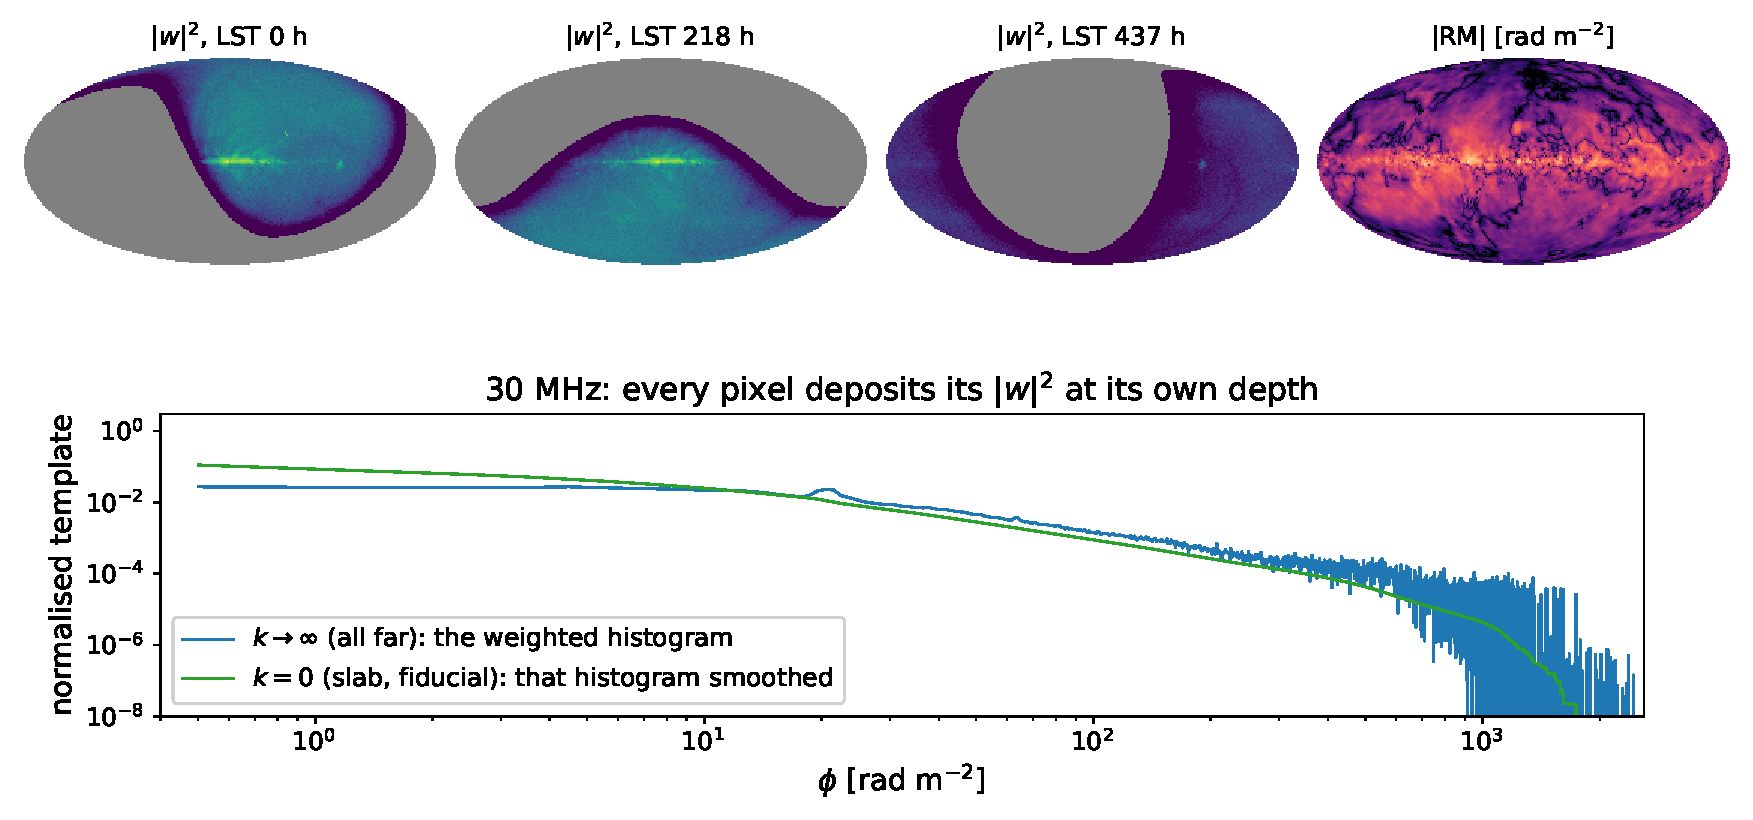
\includegraphics[width=\textwidth]{step5_inputs.pdf}
  \caption{The two inputs to Equation~\eqref{eq:deposit} and what they
  build, at 30\,MHz. Top: the beam-sky weight $|w|^2$ at three local
  sidereal times, and the Galactic Faraday depth map
  \citep{hutschenreuter2022}. Grey is sky below the horizon, which
  carries exactly zero weight; the weight sweeps across the sky as the
  Moon rotates, so no single map can stand in for the sum over $t$ ---
  one lunar sidereal day is $655.7$\,h, which is the axis these three
  samples are drawn from. Bottom: the resulting normalised template,
  Equation~\eqref{eq:histogram} in blue and its $k=0$ smoothed version
  in green. Maps are degraded for display only; every number in this
  report is computed at native nside 512.}
  \label{fig:inputs}
\end{figure}

\subsection{The emissivity geometry: the $f^k$ pushforward}
\label{sec:pushforward}

$F(\phi)$ is not the histogram of the Faraday depth map, which gives
$\phi_{{\rm col},n}$, the depth of the \emph{entire} column. Emission
partway along is rotated only by the fraction in front of it.

Parameterise position by $f\in[0,1]$, $f=0$ at the observer, and let
the synchrotron emissivity vary as $\rho(f)\propto f^{k}$. Emission
from $f$ accumulates depth $\phi = f\phi_{\rm col}$, so
\begin{align}
  \mathrm{CDF}_n(e)
  &= \Pr\bigl[f\phi_{{\rm col},n} \le e\bigr]
   = \frac{\displaystyle\int_0^{\min(e/\phi_{{\rm col},n},1)} f^{k}\,
     \mathrm df}{\displaystyle\int_0^{1} f^{k}\,\mathrm df}
   = \min\!\left(\frac{e}{\phi_{{\rm col},n}},1\right)^{k+1}.
  \label{eq:pushforward}
\end{align}
$F$ is the $|w_n|^2$-weighted sum of Equation~\eqref{eq:pushforward}
over sightlines, differenced onto bins. The condition $k \ge -1$ is
exactly integrability of $f^k$ at the origin.

Three values bracket the geometry: $k\to\infty$ (all emission at the
far end, $F$ is the weighted histogram of $\phi_{\rm col}$); $k=0$
(uniform slab, the \textbf{fiducial}); and $k\to-1$ (all local,
$F\to\delta(\phi)$). Every finite-$k$ pushforward puts mass at
$\phi = 0$, because every column has a near end.

\paragraph{What $f$ indexes.} The parameterisation sets $\phi =
f\phi_{\rm col}$, so $f$ is the fraction of the column's Faraday
\emph{depth} already accumulated, not the fraction of its physical
length. Any non-uniformity in how $\phi$ piles up along the line of
sight is absorbed into $f$ before $k$ is chosen, and $\rho(f)\propto
f^{k}$ is a statement about emissivity per unit accumulated depth. That
is weaker than ``uniform slab'' suggests: what has to be a power law is
the emissivity against depth, not against distance.

\paragraph{One histogram in, a family out.} Only $k\to\infty$ is a
histogram of anything --- it is the $|w|^2$-weighted histogram of
$|\mathrm{RM}|$ itself, and the implementation takes that code path.
Every other $k$ is that histogram passed through the smoothing operator
of Equation~\eqref{eq:pushforward}. Figure~\ref{fig:family} draws the
family; Table~\ref{tab:mass} counts it.

\begin{figure}[htbp]
  \centering
  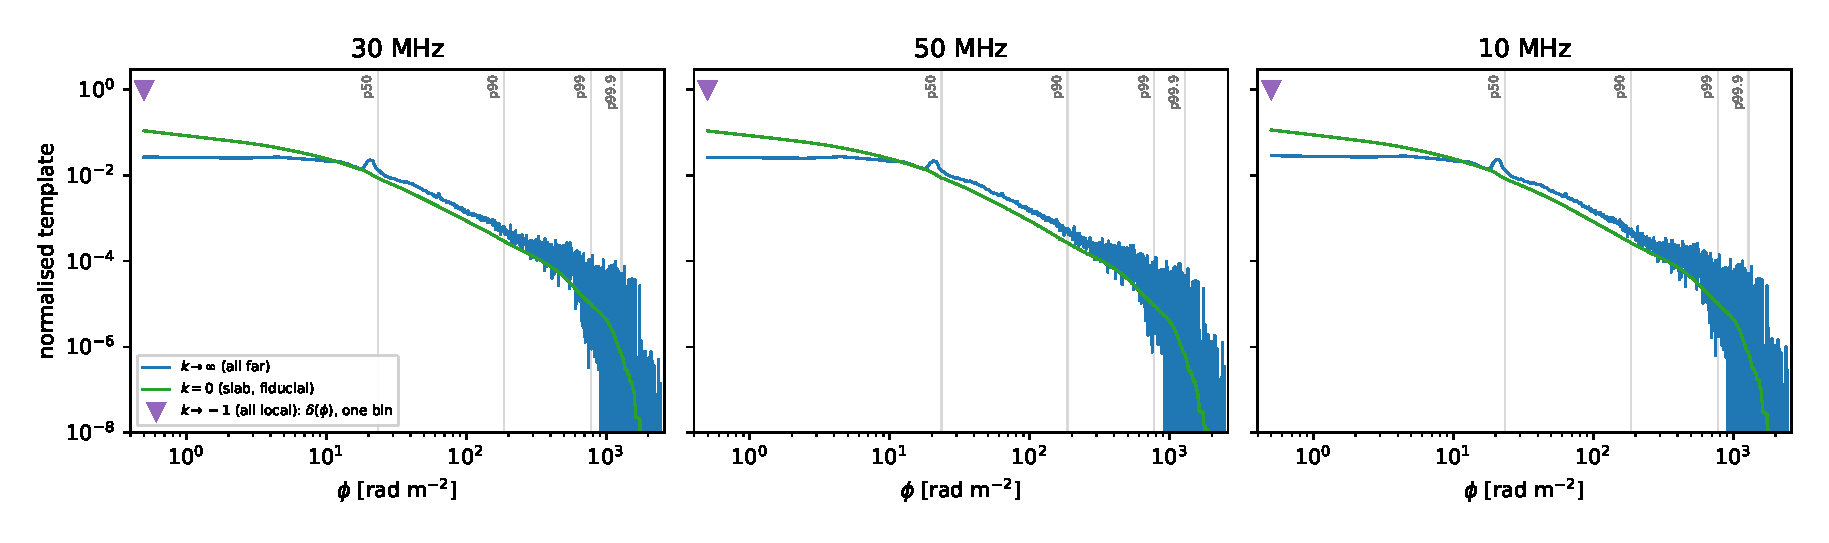
\includegraphics[width=\textwidth]{step5_template_family.pdf}
  \caption{The normalised template for three bands and the emissivity
  geometries of this section. Colour is the geometry and linestyle the
  treatment. \textbf{$k\to\infty$ (blue) is the sky's own
  $|w|^2$-weighted $|\mathrm{RM}|$ histogram; every other geometry is
  that histogram smoothed} by Equation~\eqref{eq:pushforward} --- which
  is visible directly, the $k\to\infty$ curve going ragged above
  $\sim300$\,\rmu{} where its bins hold few pixels while $k=0$ stays
  smooth, each column there contributing to every bin below it.
  $k\to-1$ is $\delta(\phi)$ by construction and is marked rather than
  drawn.}
  \label{fig:family}
\end{figure}

\begin{table}[htbp]
  \centering
  \caption{Where the template mass sits at \MassBand\,MHz: the
  normalised folded template summed over depth bands, per geometry.
  The columns total to one because the pushforward \emph{redistributes}
  power in depth rather than reweighting it. Units of $\phi$ are
  \rmu.}
  \label{tab:mass}
  \begin{tabular}{lccc}
    \toprule
    $\phi$ band & $k\to\infty$ & $k=0$ (fiducial) & $k\to-1$ \\
    \midrule
    \MassRows
    \bottomrule
  \end{tabular}
\end{table}

Every column keeps its $|w|^2$ and only its position on the depth axis
moves. What changes is where that power sits: the fiducial geometry
carries \MassZeroBinFid\% of the template mass in the lowest bin
against \MassZeroBinInf\% for the screen, and that is precisely the
mass degenerate with the smooth leakage Section~\ref{sec:detection}
cuts away. Assuming $k\to\infty$ would have overstated the power
surviving the cut by $\kscanSpanHiThirty\times$.

\paragraph{Why it smooths.} For the fiducial geometry the pushforward
has a closed form. A column at depth $x$ lays down uniform density
$1/x$ over $[0,x]$, so with $h$ the $|w|^2$-weighted histogram of
$|\phi_{\rm col}|$,
\begin{equation}
  F_0(\phi) \;=\; \int_{x>\phi} \frac{h(x)}{x}\,\mathrm dx .
  \label{eq:survival}
\end{equation}
$F_0$ is a \emph{survival integral} of $h$ --- not a convolution with a
fixed kernel, but a cumulative integral whose weight $1/x$ falls with
depth. An integral of a ragged function is smooth and monotone however
ragged the function is, which is why the $k\to\infty$ curve of
Figure~\ref{fig:family} is visibly noisy in its tail while every finite
$k$ is not.

\paragraph{When it broadens, and when it narrows.} The initial fall of
the channel covariance is set by the variance of $F$
(Section~\ref{sec:roadmap}), so the \emph{sign} of the geometry's
effect follows from what the pushforward does to that variance. Write
$\phi = fX$ with $X = \phi_{\rm col}$ and $f$ the emissivity variable
of Equation~\eqref{eq:pushforward}, independent of $X$. Then
\begin{equation}
  \operatorname{Var}(fX) =
  \mathbb{E}[f^2]\,\mathbb{E}[X^2] - \mathbb{E}[f]^2\mu^2,
  \qquad
  \operatorname{Var}(X) = \mathbb{E}[X^2] - \mu^2,
  \label{eq:pushvar}
\end{equation}
with $\mu = \mathbb{E}[X]$; for $\rho(f)\propto f^k$,
$\mathbb{E}[f] = \tfrac{k+1}{k+2}$ and
$\mathbb{E}[f^2] = \tfrac{k+1}{k+3}$. At the fiducial $k=0$ these are
$\tfrac12$ and $\tfrac13$, and the two variances are equal when
$\mathbb{E}[X^2]/\mu^2 = 9/8$ --- that is, at a coefficient of
variation
\begin{equation}
  \mathrm{CV} \;\equiv\; \frac{\sqrt{\operatorname{Var}(X)}}{|\mu|}
  \;=\; \sqrt{\tfrac18} \;=\; 0.354 .
  \label{eq:cvcrit}
\end{equation}

Below that the pushforward \textbf{broadens} $F$; above it, it
\textbf{narrows} it. Multiplying by $f<1$ shrinks the depths, which
reduces spread, while the randomness of $f$ adds spread; which wins
depends on whether $X$ already has spread of its own to shrink. A
single screen has $\mathrm{CV}=0$ and can only be broadened. The
Galactic sky is heavy-tailed, $\mathbb{E}[X^2]\gg\mu^2$, and
Equation~\eqref{eq:pushvar} tends to
$\operatorname{Var}(fX)/\operatorname{Var}(X)\to\tfrac13$: \textbf{the
fiducial geometry makes the template narrower than the map's own
histogram}, so its covariance decorrelates more slowly, not faster.
The geometry is therefore not a monotone knob --- its sign of effect
flips at Equation~\eqref{eq:cvcrit}. Measured on the beam-weighted sky,
$\mathrm{CV} = \cvHutschenreuter$ and
$\operatorname{Var}(fX)/\operatorname{Var}(X) = \cvVarRatioHutschenreuter$,
within a per cent of the $1/3$ asymptote. Figure~\ref{fig:twoaxes}
draws both axes together: a constant RM map ($\mathrm{CV}=\cvConstant$)
is $\delta(\phi_0)$ at $k\to\infty$ and a top hat at $k=0$, the same sky
giving opposite covariances, which is what makes the two axes
independent.

\begin{figure}[htbp]
  \centering
  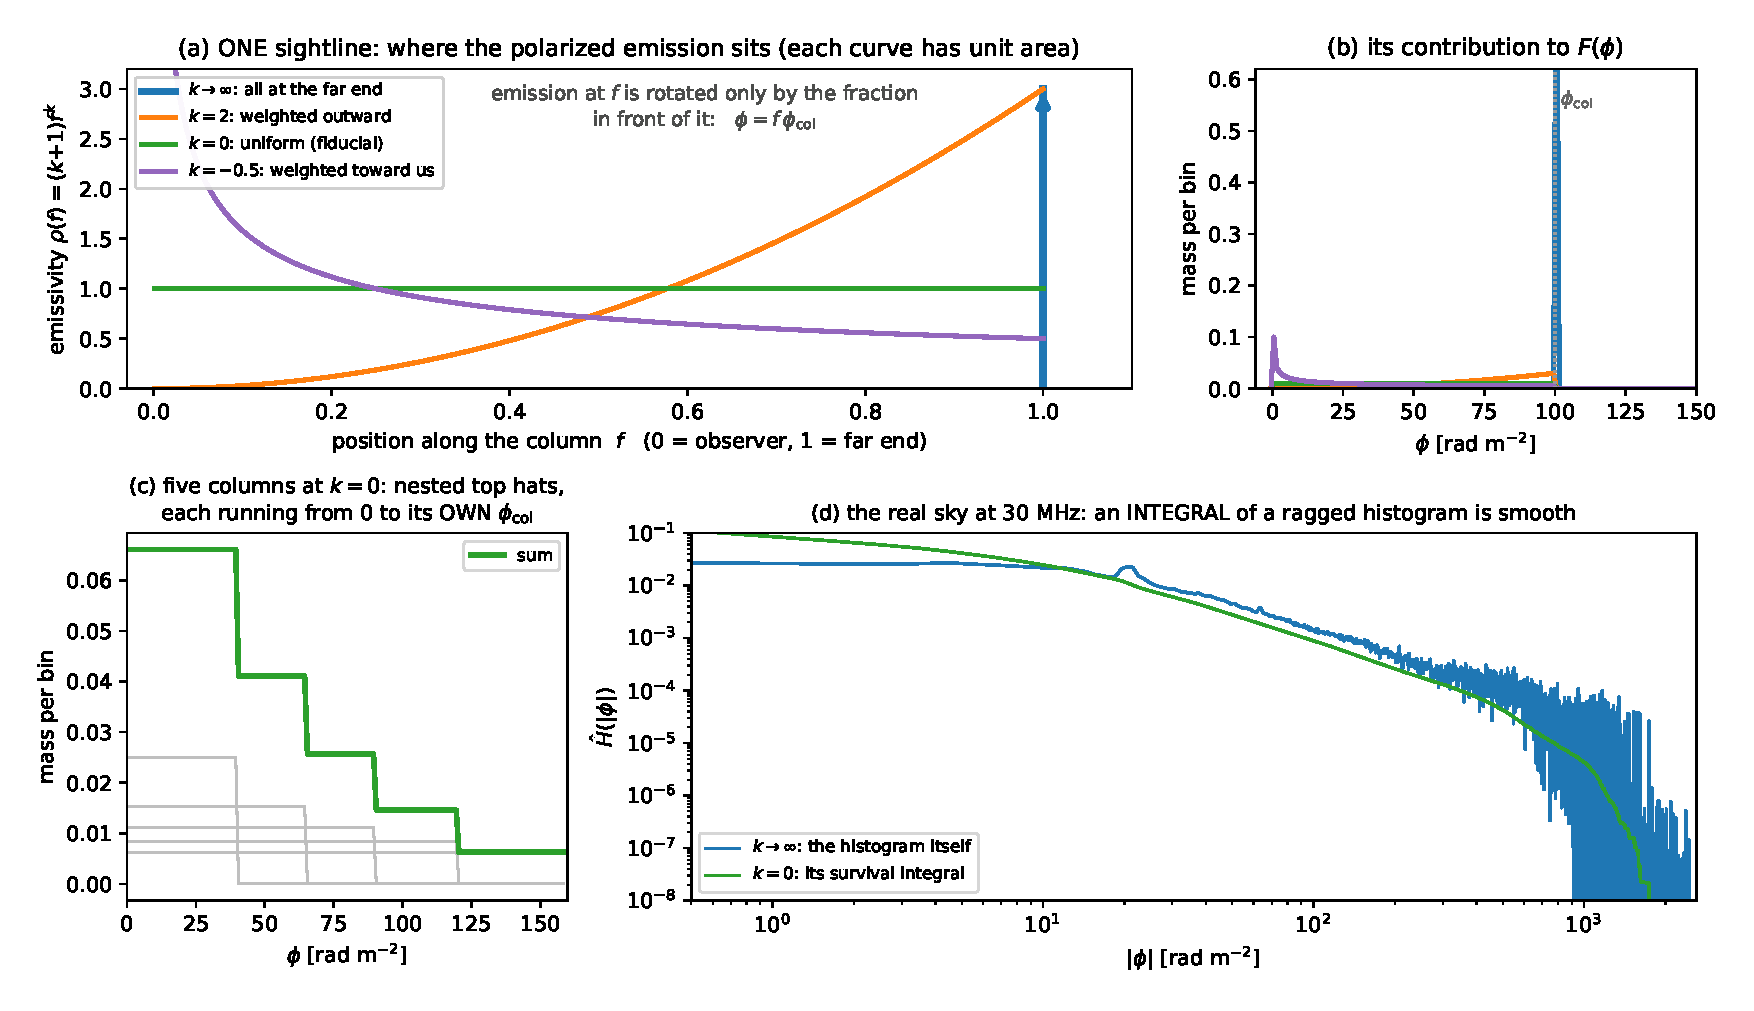
\includegraphics[width=\textwidth]{step5_pushforward.pdf}
  \caption{How the pushforward mixes emission. (a) One sightline under
  four geometries; each curve carries unit area. (b) What that single
  sightline deposits in depth --- a delta at $\phi_{\rm col}$ for the
  screen, a top hat for the slab. (c) Five columns at $k=0$: nested top
  hats, each running from zero to its \emph{own} $\phi_{\rm col}$.
  (d) The real sky: because Equation~\eqref{eq:survival} is an integral
  of the histogram, the result is smooth and monotone however ragged
  the histogram is.}
  \label{fig:pushforward}
\end{figure}

\begin{figure}[htbp]
  \centering
  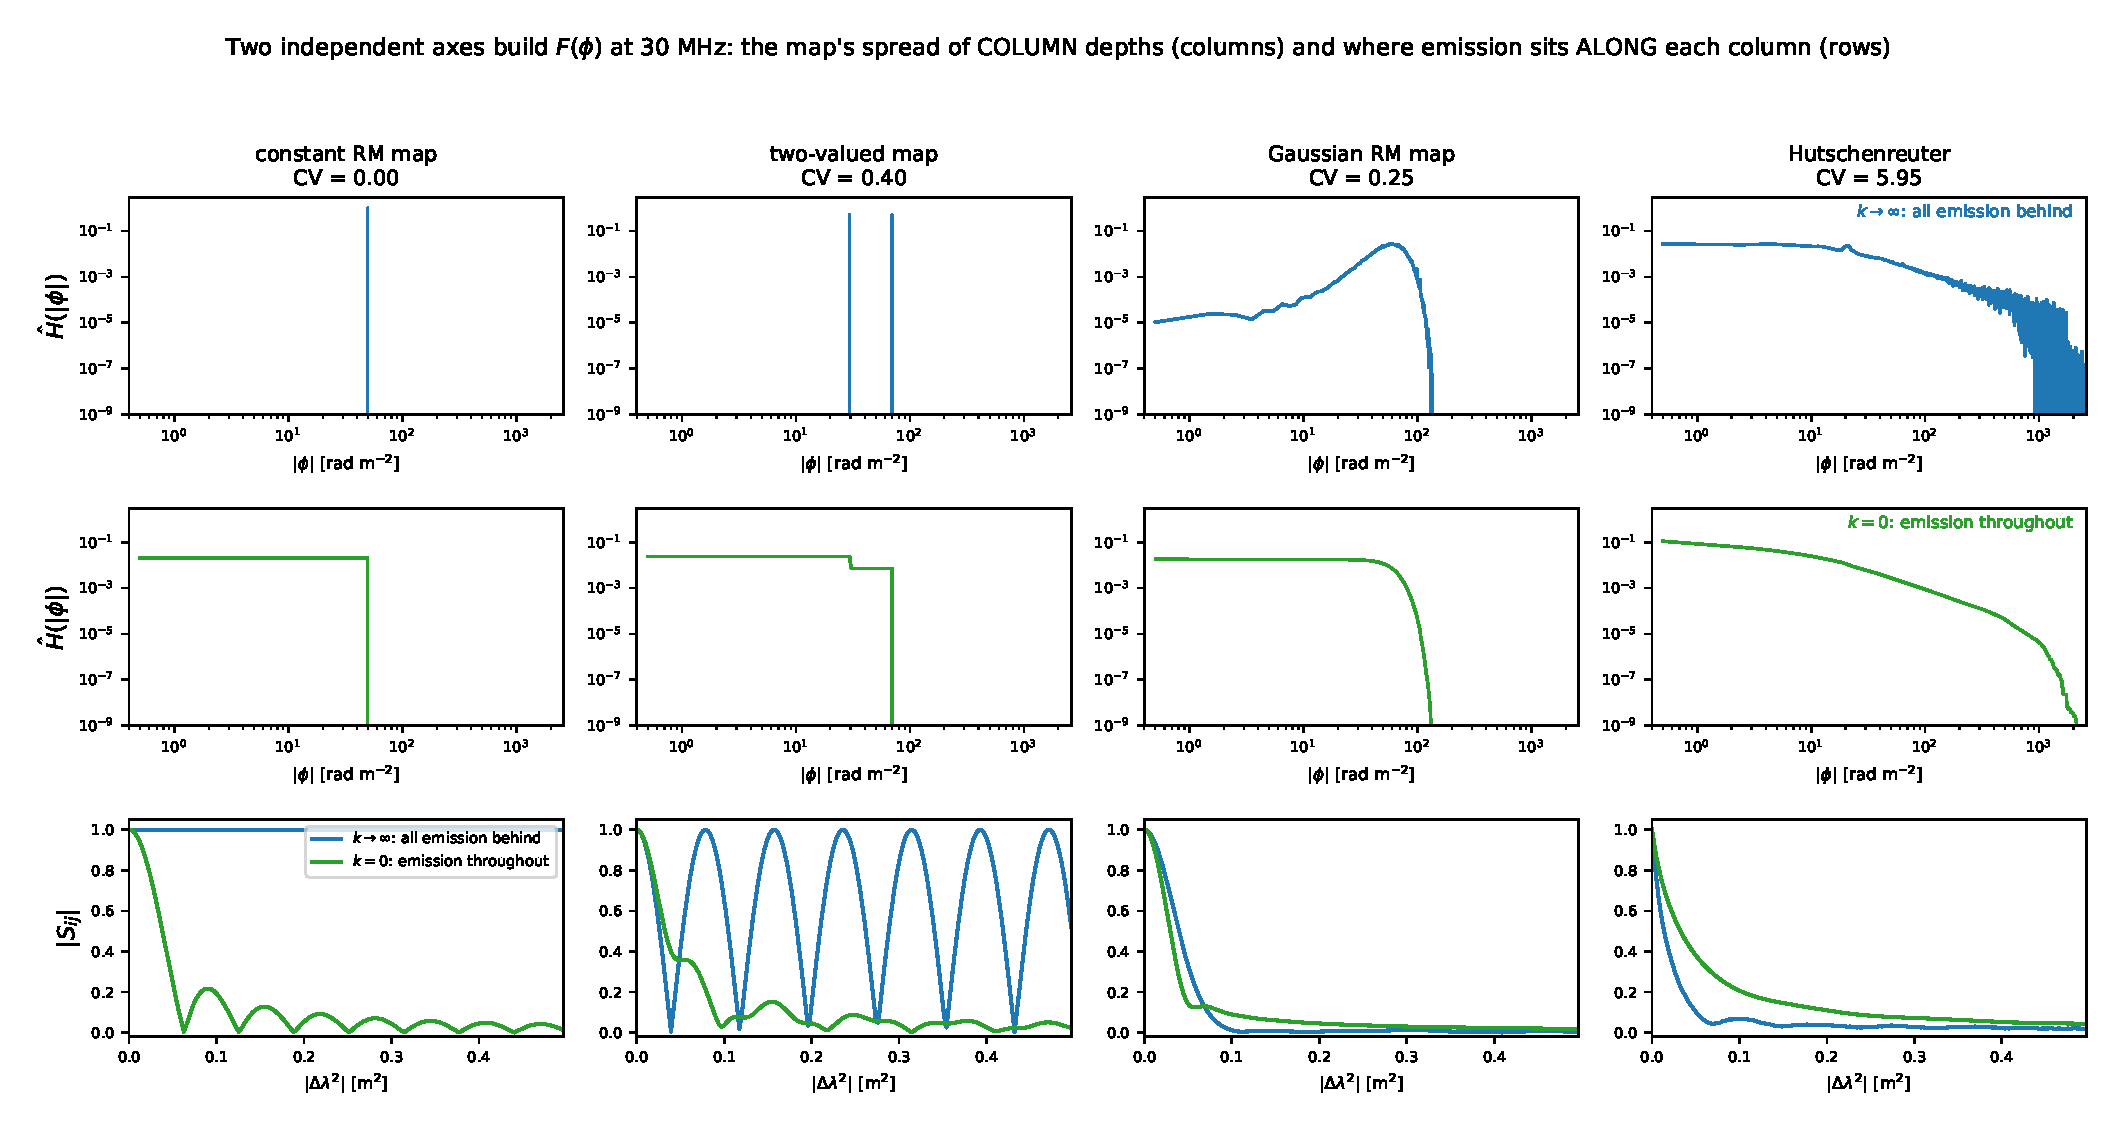
\includegraphics[width=\textwidth]{step5_two_axes.pdf}
  \caption{The two axes that build $F$, and what each does to the
  covariance. Columns are the map's spread of \emph{column} depths;
  rows are where emission sits \emph{along} each column. Column one is
  the proof they are independent: one constant RM map is
  $\delta(\phi_0)$ at $k\to\infty$ and a top hat at $k=0$, with
  opposite covariances. Note the effect of $k$ on $|S|$ reverses
  between the first column and the last, at the coefficient of
  variation of Equation~\eqref{eq:cvcrit}. Each panel depends on its
  map only through the weighted histogram, never the arrangement, which
  is why an alternating checkerboard is a legitimate two-valued sky.}
  \label{fig:twoaxes}
\end{figure}

\paragraph{$F$ sees only a histogram.} Equation~\eqref{eq:deposit}
contains no pixel position: each pixel deposits its weight in the bin
holding its depth and nothing else. $F$ therefore depends on the map
only through the joint distribution of (weight, depth) over pixels, and
not at all on how those pixels are arranged on the sky. Two
consequences follow. The acceptance gate's rigid rotation
(Section~\ref{sec:gates}) is a pixel permutation and leaves the
statistic invariant by construction whenever the weights are uniform.
And the RM map's spatial power spectrum is discarded entirely --- which
is the deeper reason $\theta_c$ cannot be recovered from the template
(Section~\ref{sec:clamp}).

\paragraph{The sightline spread is not a substitute.} The sky already
supplies a wide range of depths, one per column, so it is fair to ask
what the pushforward adds. The difference is structural. The sightline
mixture places every column at a single $\phi_{{\rm col},n}$ and has no
mechanism to put it anywhere else; the pushforward drags mass to zero
depth from \emph{every} column, however deep. A sky with all
$|\mathrm{RM}|>500$ would give an $F_{\infty}$ supported entirely above
$500$ and an $F_{0}$ supported down to the origin. Nor is the
difference a rescaling of the axis: the best squeeze factor mapping
$F_{\infty}$ onto $F_{0}$ is $\kscanSqueezeThirty$ and still leaves a
Kolmogorov distance of $\kscanSqueezeKSThirty$ (against
$\kscanRawKSThirty$ unrescaled), an order of magnitude outside the
$10^{-2}$ tolerance this report uses for shape agreement.

\subsection{How much the geometry decides}
\label{sec:kscan}

Three geometries do not show the \emph{shape} of the dependence, and
that shape is the robustness claim. Figure~\ref{fig:kscan} scans $k$
continuously. It re-casts the stored $k\to\infty$ histogram rather than
re-running the template job, which is legitimate because that histogram
is exactly the pushforward's input; the reconstruction reproduces the
stored $k=0$ column to a Kolmogorov distance of \kscanKSThirty{} and
its detection ratio to \kscanRatioZeroThirty{} against the
\detSafeSlabThirty{} of Table~\ref{tab:detection}, arrived at by an
independent path.

\begin{figure}[htbp]
  \centering
  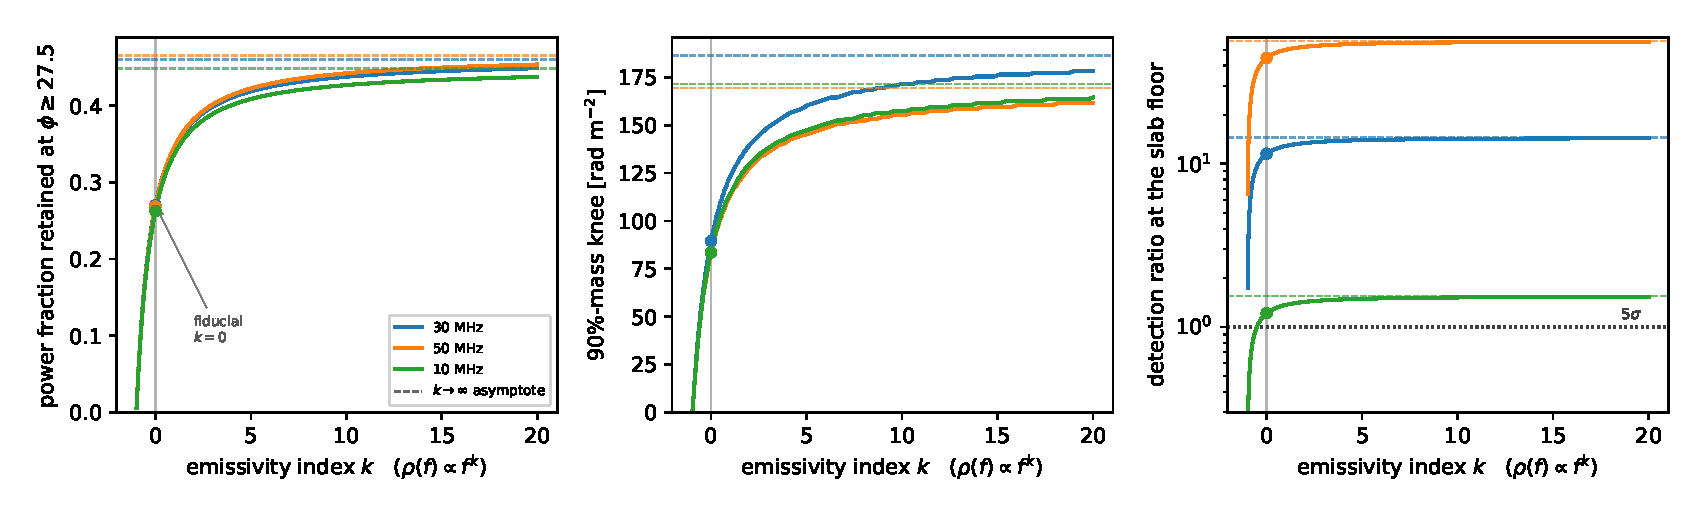
\includegraphics[width=\textwidth]{step5_kscan.pdf}
  \caption{The emissivity geometry as a continuous knob: retained power
  above the systematics cut, the 90\%-mass knee, and the detection
  ratio at the slab floor. Dashed is the $k\to\infty$ asymptote, which
  cannot sit on a linear $k$ axis; $k\to-1$ is off the left edge by
  construction. The threshold in the right panel is recomputed on the
  truncated template at every $k$.}
  \label{fig:kscan}
\end{figure}

The dependence is \textbf{shallow above $k=0$ and steep only as
$k\to-1$}. Over $k\in[0,\infty)$ --- emissivity flat or rising outward
--- the retained fraction moves by $\kscanSpanHiThirty\times$ at
30\,MHz, which is $\kscanAmpThirty\times$ in amplitude, so the
detection ratio runs \kscanRatioZeroThirty{} to \kscanRatioInfThirty.
Over $k\in[\kscanKLow,0]$ it moves by $\kscanSpanLoThirty\times$.
Almost all of that flows through the retained fraction and not the
threshold: the matched filter is integrating a distribution spanning
hundreds of resolution elements, and moving mass around inside that
support barely changes how well a broadband filter does against it.

The roll-off statistic in the middle panel is the \textbf{90\%-mass
quantile} of the folded template --- a CDF quantile, not a half-power
crossing, because a half-power statistic pins to the narrow spike the
$k=0$ slab piles up at the origin.

The emissivity geometry is therefore a factor-\kscanAmpThirty{}
systematic on the detection number, and it changes no verdict of
Section~\ref{sec:detection}. Set against the factor \floorRatioThirty{}
between the two depolarisation floors of
Section~\ref{sec:bracket}, it is subdominant --- which is the substance
of the claim that the science case turns on the floor and not on the
template.

\subsection{How robust the shape is to the sky and the instrument}
\label{sec:robust}

Section~\ref{sec:kscan} perturbed the emissivity geometry. Two
further perturbations act on the inputs rather than on the model:
the sky weighting and the instrument arm.

\begin{table}[htbp]
  \centering
  \caption{The 90\%-mass knee at $k=0$ under two perturbations. Units
  \rmu.}
  \label{tab:robust}
  \begin{tabular}{lccccc}
    \toprule
    Band & knee & plane-tapered & taper factor & two-port arm & arm swap \\
    \midrule
    \RobustnessRows
    \bottomrule
  \end{tabular}
\end{table}

\paragraph{Plane taper.} Down-weighting the Galactic plane by
$\sin^2|b|$ moves the knee by a factor $\taperFactorThirty$ at 30\,MHz,
so \textbf{the roll-off is carried by the plane}. That is the
\emph{unfavourable} branch: long in-plane paths are where
$B_\parallel$ reverses and the linear $\phi(f)$ ansatz of
Section~\ref{sec:pushforward} is weakest, so \textbf{the amplitude
bracket must be read as wider, not narrower}, than
Table~\ref{tab:bracket} suggests. The direction of the reversal effect
is favourable --- reversals broaden $F$ outward --- but its size is not
bounded by anything computed here.

\paragraph{Compact sources.} The weighting is dominated by extremes:
the brightest $0.01\%$ of pixels carry $\weightConc\%$ of the template
weight. The brightest polarized pixel in the WMAP K map lies
$\crabSep^\circ$ from Taurus A, and within one degree of the Crab
$\crabSkyPct\%$ of the sky carries $\crabWeightPct\%$ of all weight at
$\crabContrast\times$ the mean polarized brightness. Because the map
puts that region at $|\phi|\approx20$\,\rmu, it is what produces the
local excess visible in the $k\to\infty$ curve of
Figures~\ref{fig:inputs} and~\ref{fig:family}: measured at
$\crabExcess\times$ a local smooth, falling to $\crabExcised\times$ when
the region is excised. It is not instrumental --- the two arms agree ---
and at the fiducial geometry the pushforward has already smoothed it
away, which is why the $k=0$ curve shows no such feature.

This report does \emph{not} mask it. Masking compact polarized sources
is a decision for the sky model, and a source-subtracted polarization
map is the principled fix; what belongs here is the bound. Excising the
region moves the knee by $\crabKneePct\%$ and the detection ratio by
$\crabRatioPct\%$.

\paragraph{Two arms.} Swapping the four-port $|w|^2$ for the symmetric
two-port one moves the knee by $\armSwapFifty$\% at 50\,MHz and
$\armSwapTen$\% at 10\,MHz, but only $\armSwapThirty$\% at 30\,MHz. The
beams weight different declination strips; at the band that owns the
knee they agree. Figure~\ref{fig:twoarm} shows the templates.

\begin{figure}[htbp]
  \centering
  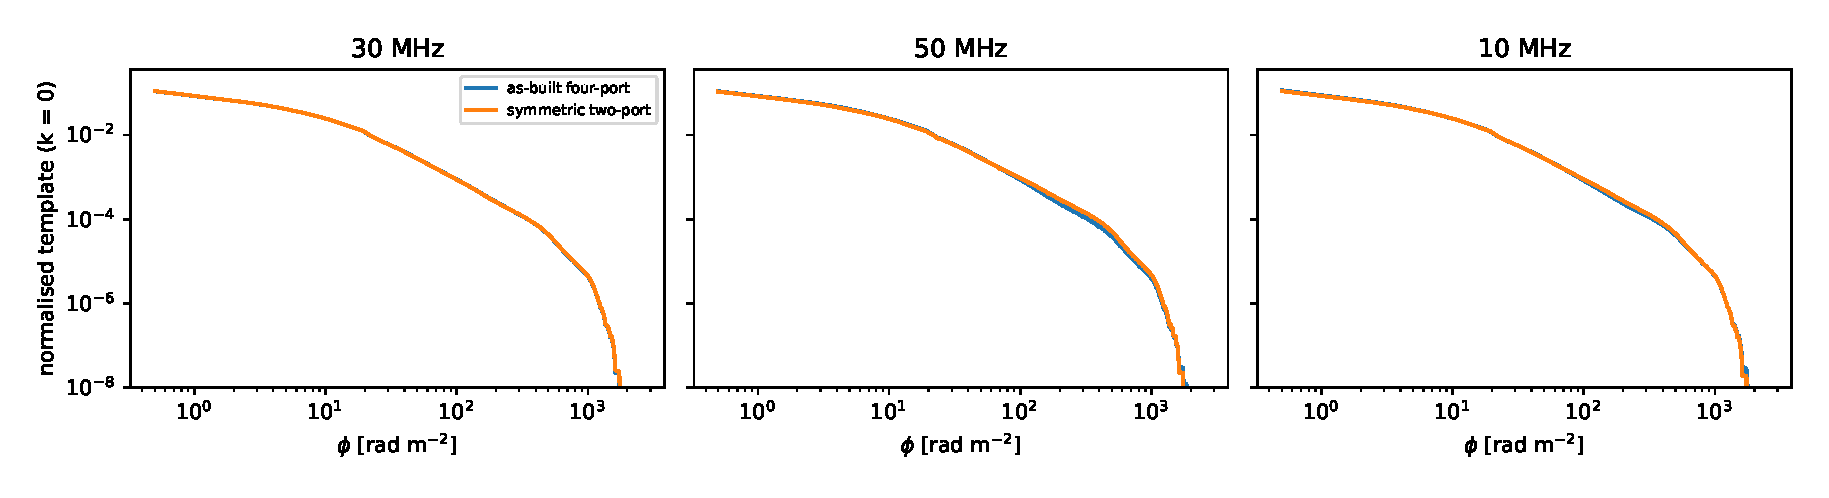
\includegraphics[width=\textwidth]{step5_two_arm.pdf}
  \caption{The $k=0$ template through the as-built four-port response
  and the symmetric two-port pseudo-dipole.}
  \label{fig:twoarm}
\end{figure}

\subsection{The acceptance gates}
\label{sec:gates}

The normalised $F(\phi)$ moves by Kolmogorov distances of
$2\times10^{-5}$ to $1.9\times10^{-4}$ across nside 256--2048 and under
a rigid null rotation, against a $10^{-2}$ tolerance, while the
coherent observable collapses by $134\times$ under the same refinement
and moves by $7.2\times$ under the rotation alone.

These gates do \emph{not} test Section~\ref{sec:identity}: with the
uniform weights they use, a rigid rotation is a pixel permutation that
leaves the statistic invariant by construction, and the nside 1024 and
2048 legs are interpolated upsamplings carrying no new sky.

\subsection{What the template is for}
\label{sec:roadmap}

$F(\phi)$ is now built, and the rest of this report does exactly three
things with it.

\textbf{It becomes a frequency covariance, not a spectrum.} The
temptation is to transform $F$ once through
Equation~\eqref{eq:rmsynth} and compare $P(\lamsq)$ against data. That
is the wrong object here for the same reason
Section~\ref{sec:randomwalk} gave: the intrinsic phases are unknown, so
$P(\lamsq)$ has an unpredictable phase and only its second moment is
predictable. The signal is therefore modelled as a Gaussian field of
known normalised shape and unknown amplitude, whose covariance between
two channels is Equation~\eqref{eq:rmsynth} evaluated at their
\emph{separation} rather than at either channel,
\begin{equation}
  S_{ij} \;=\; \sum_b \hat H_b\, e^{2i\phi_b(\lamsq_i - \lamsq_j)}
  \;=\; P\bigl(\lamsq_i - \lamsq_j\bigr) ,
  \label{eq:sij}
\end{equation}
with $\hat H$ the normalised template. Nothing is discarded in the step
from $F$ to $S$: Equation~\eqref{eq:sij} is the same transform, read on
the difference axis.

\textbf{It is measured through a real instrument.}
Section~\ref{sec:resolution} carries a unit tone through the true
spectrometer bin weights to get the point-spread function $R$ that
Equation~\eqref{eq:identity} already invoked, the depth horizon beyond
which the channel width attenuates, and the low-depth cut that
separates the signal from smooth $I\!\to\!Q,U$ leakage.

\textbf{It is weighed against noise.} Section~\ref{sec:noise} whitens
Equation~\eqref{eq:sij} by the zoom-bin noise covariance and reads off
the amplitude at which the whole template would be a $5\sigma$
detection; Section~\ref{sec:bracket} supplies the amplitude the sky
plausibly has, which this report does not predict and quotes as a
bracket. Section~\ref{sec:detection} is the comparison of the two, and
is the deliverable.

% The basis argument is a defence of a choice, not a step in the
% construction, so it is an appendix; this keeps the main line running
% template -> instrument -> noise -> detection.
\section{What LuSEE-Night measures}
\label{sec:data}

Nothing above predicts a spectrum, and it is worth being concrete about
what it does predict and what the instrument returns.

The polarimeter delivers pseudo-Stokes $I,Q,U,V$ per channel
(\code{polarimeter.pseudo\_stokes}), so each frequency carries $Q$ and
$U$ as two independent real numbers --- equivalently the complex
$P(\nu) = Q + iU$ on which Equation~\eqref{eq:faraday} acts. That is
the data vector, and it settles a convention that matters: the
covariance of Equation~\eqref{eq:sij} is built on the \emph{signed}
depth distribution and the Fisher information of
Equation~\eqref{eq:mf} carries no factor of one half. Treating the
observable as a single real projection would discard $U$ and cost a
factor $\sqrt2$ in signal-to-noise.

Figure~\ref{fig:data} shows what follows. A single Faraday depth winds
the polarization angle linearly in \lamsq; no Faraday rotation leaves
it constant, so $Q$ and $U$ are flat; the Galactic sky decorrelates,
so they wander on the scale $|S_{ij}|$ sets. \textbf{That is the whole
observational signature} --- not a line, not a peak, but structure in
$Q$ and $U$ with a specific correlation length.

\begin{figure}[htbp]
  \centering
  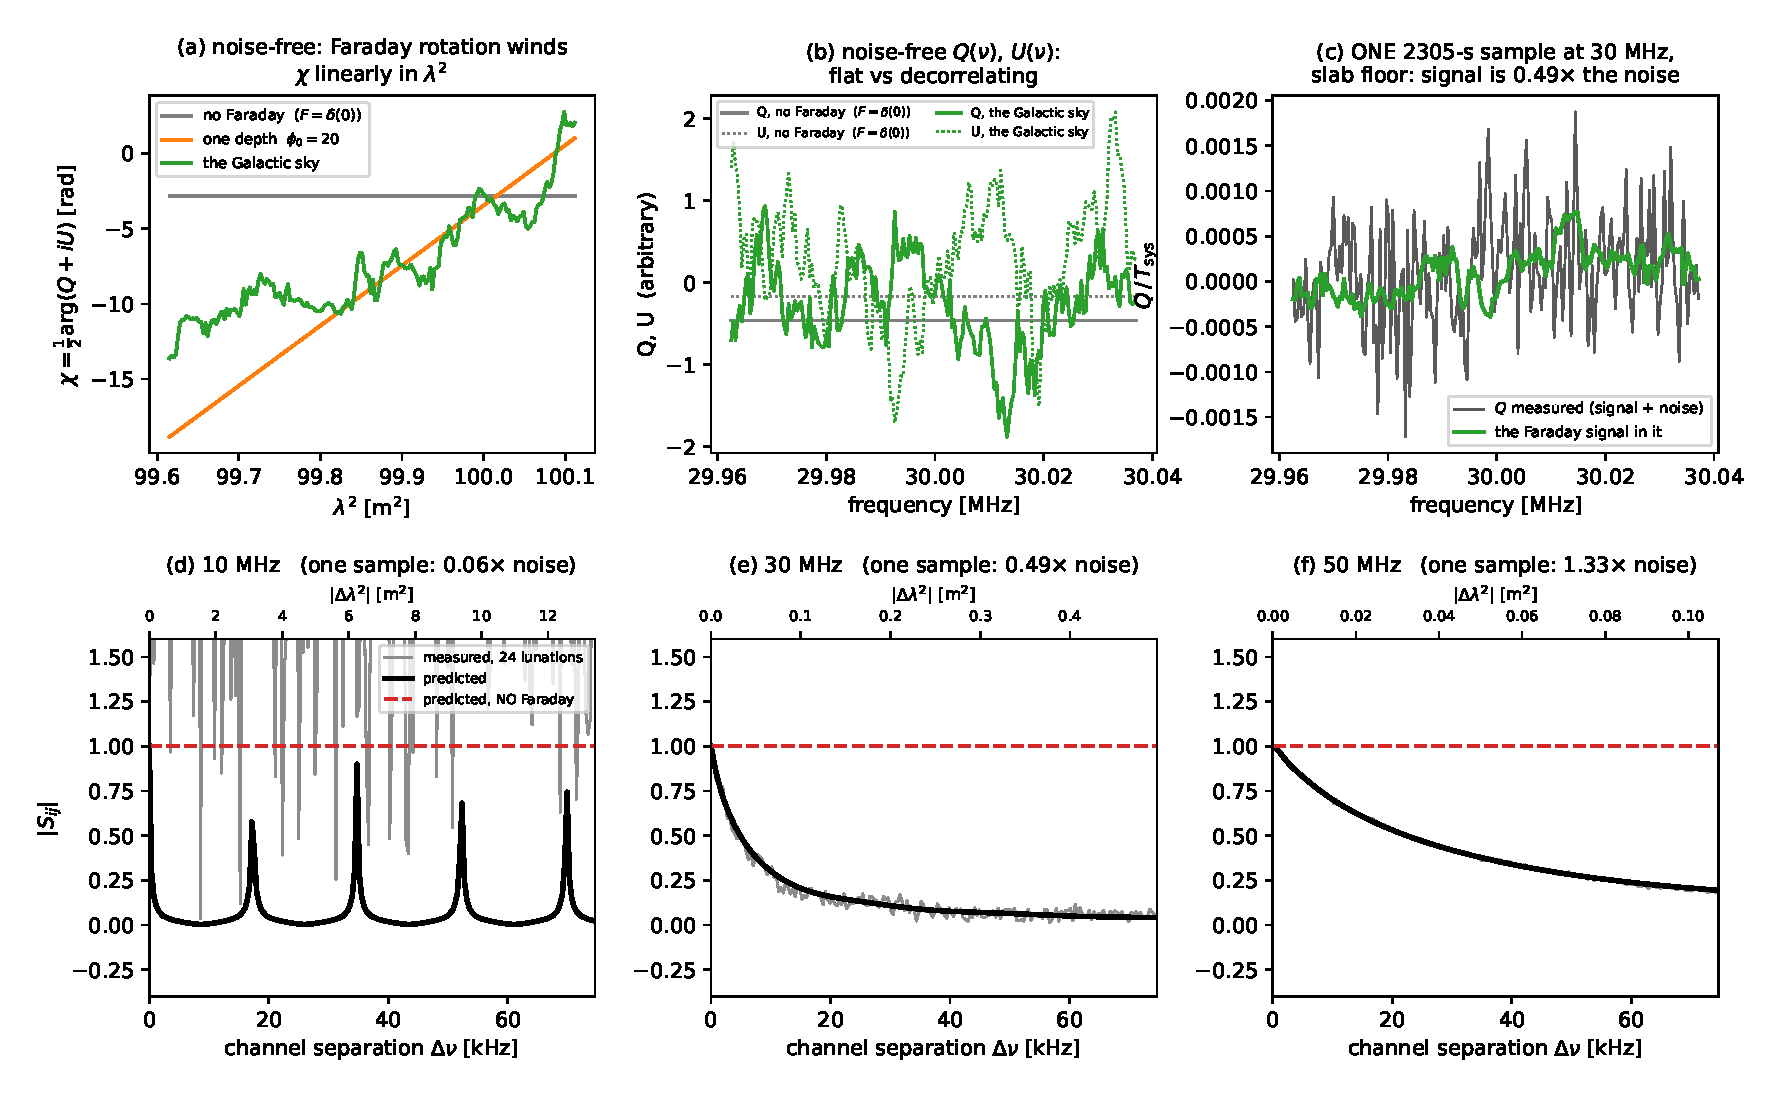
\includegraphics[width=\textwidth]{step5_data.pdf}
  \caption{What the instrument measures, drawn from this report's own
  signal model. Top row is 30\,MHz and is illustrative: (a) and (b) are
  noise-free, and (c) is one sample at the uniform-slab floor, where
  the signal is a fraction of the noise. No single spectrum is a
  detection and none is meant to be. The bottom row is the object
  actually predicted, at all three bands, against \emph{frequency}
  separation with \lamsq{} on the opposite axis. Coadding drives the
  measured covariance onto $|S_{ij}|$; the no-Faraday hypothesis is the
  flat line at unity. The three bands differ in kind, not degree:
  50\,MHz has the best single-sample sensitivity but spans only
  $0.10\,\mathrm{m^2}$ in \lamsq{} and so barely decorrelates across
  the band; 10\,MHz is aliased --- the periodic revivals are template
  power folding back past the depth-Nyquist wall
  (Appendix~\ref{sec:bases}) --- and its single samples are
  noise. 30\,MHz is the band where the decorrelation is both large and
  clean.}
  \label{fig:data}
\end{figure}

So the analysis chain is: measure $Q(\nu)$ and $U(\nu)$, form
$P = Q+iU$, estimate its channel covariance across the mission, and
test that covariance against $S$. Section~\ref{sec:noise} is the
optimal version of that test.

\paragraph{Zoom mode throughout.} Every covariance in this report is
built on the \textbf{zoom} channelisation --- $192$ bins of
$390.625$\,Hz --- through luseepy's real spectrometer response, not a
boxcar (\code{dispersion.zoom\_bin\_matrix}). That is not a free
choice: Section~\ref{sec:horizon} shows no parent bin reaches the
knee, so the parent mode cannot see the signal at all, and no
parent-mode detection number is computed anywhere here. The
parent/zoom comparison appears once, in Figure~\ref{fig:envelope},
and it is what justifies the choice rather than an aside.

\subsection{How much the prediction depends on inputs we do not
control}
\label{sec:inputsens}

$S$ is built from the RM map, the polarized emissivity, the beam and
the emissivity geometry. Only one of them matters.

\begin{figure}[htbp]
  \centering
  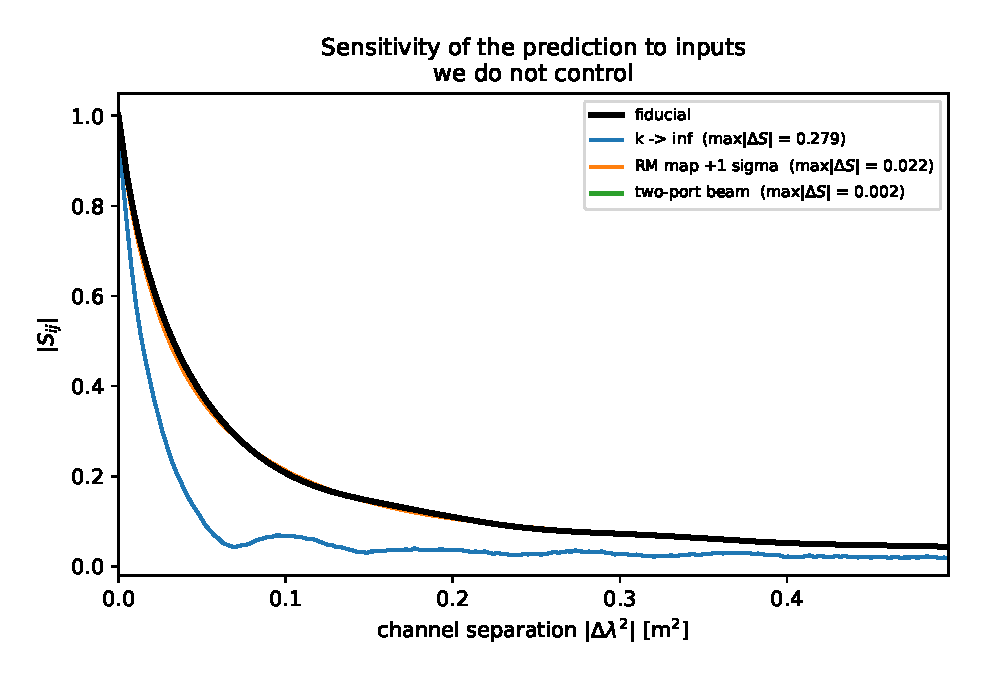
\includegraphics[width=0.62\textwidth]{step5_robustness.pdf}
  \caption{Sensitivity of $|S_{ij}|$ to its inputs. Everything except
  the emissivity geometry lies on the fiducial curve.}
  \label{fig:robustness}
\end{figure}

Perturbing the geometry from $k=0$ to $k\to\infty$ moves $|S|$ by
$\dSKInf$. Redrawing the RM map at its own stated $1\sigma$ --- a
median uncertainty of \rmStdMedian\,\rmu{} against a median $|{\rm
RM}|$ of \rmAbsMedian, i.e. \rmStdPct\% --- moves it by $\dSRmSigma$,
because adding that much scatter to a distribution of coefficient of
variation \cvHutschenreuter{} is a small perturbation. Swapping the
four-port beam for the two-port one moves it by $\dSTwoPort$.

The WMAP spectral index cannot move it at all, and that is exact rather
than measured: $(\nu/\nu_{\rm ref})^\beta$ is a spatially \emph{uniform}
rescaling of the emissivity, so it multiplies $|w|^2$ by a constant and
cancels in the normalised template (measured residual $\betaShift$).
Only the spatial \emph{pattern} of the polarized sky enters, never its
overall scale or spectral index. A spatially \emph{varying} index would
reweight pixels against each other and is not tested here.

Two caveats travel with this. The RM redraw uses independent per-pixel
noise, whereas the reconstruction's errors are correlated; the coherent
limit is benign for $|S|$, which is exactly invariant under a uniform
depth shift, but not for the threshold. And $\sigma_{\rm eff}$ appears
in Section~\ref{sec:bracket} as an amplitude and nowhere in $F$ ---
if that turbulence exists it should broaden the template too, which
Section~\ref{sec:cannot} takes up.

\section{What sets the template, and the cut}
\label{sec:resolution}

\subsection{The point-spread function}
\label{sec:rmsf}

The instrument samples \lamsq{} at its spectrometer bin centres --- for
the zoom mode, 192 bins spaced $390.625$\,Hz apart spanning
$74\,609$\,Hz. For ideal top-hat coverage of a \lamsq{} span
$\Delta\lamsq$ the response to a unit tone is
\begin{equation}
  R(\phi) = \operatorname{sinc}\bigl(\phi\,\Delta\lamsq\bigr),
  \qquad \operatorname{sinc}x = \frac{\sin x}{x}.
  \label{eq:rmsfideal}
\end{equation}
The implementation does not assume this: it carries a unit tone through
the \emph{true} bin weight matrix and transforms over the bin centres.

Two conventions must travel with any width. The implementation returns
\emph{power}, so a width read off it is a power FWHM; the conventional
RM-synthesis resolution is an \emph{amplitude} FWHM. For the sinc,
$|\operatorname{sinc}x| = 1/\sqrt2$ at $x=1.3916$ and $1/2$ at
$x=1.8955$, so
\begin{equation}
  \frac{\text{power FWHM}}{\text{amplitude FWHM}}
  = \frac{1.3916}{1.8955} = 0.734,
  \qquad
  \text{amplitude FWHM}_{\rm ideal} = \frac{2\times1.8955}{\Delta\lamsq}.
  \label{eq:conventions}
\end{equation}

\begin{table}[htbp]
  \centering
  \caption{Faraday resolution from the true zoom-bin responses. Both
  FWHM columns are measured independently, not related by
  Equation~\eqref{eq:conventions}. Units \rmu.}
  \label{tab:rmsf}
  \begin{tabular}{lccc}
    \toprule
    Band & power FWHM & \textbf{amplitude FWHM} & ideal top-hat, same span \\
    \midrule
    \ResolutionRows
    \bottomrule
  \end{tabular}
\end{table}

The measured response sits $0.5\%$ \emph{below} the ideal top-hat of
the same span, at exactly $191/192$ of it --- the $(n-1)/n$ correction
for summing $n=192$ discrete samples instead of integrating.
\textbf{The real bin responses do not broaden the point-spread function
at all}; they attenuate, which is Section~\ref{sec:horizon}.

\subsection{Channel width as a depth horizon}
\label{sec:horizon}

A spectrometer bin is a window in $\nu$, hence a multiplicative
envelope in depth: for normalised bin response $w(\nu)$,
\begin{equation}
  E(\phi) = \left|\int w(\nu)\,
  e^{2i\phi[\lamsq(\nu)-\lamsq_0]}\,\mathrm d\nu\right|,
  \label{eq:envelope}
\end{equation}
the modulus of the bin response's Fourier transform at that depth's
Faraday rate. The \emph{depth horizon} is where $E$ falls through
$\tfrac12$.

\begin{table}[htbp]
  \centering
  \caption{Depth horizons against the beam-weighted sky. Units \rmu.}
  \label{tab:horizon}
  \begin{minipage}{0.46\textwidth}
    \centering
    \begin{tabular}{lcc}
      \toprule
      Band & parent horizon & zoom horizon \\
      \midrule
      \HorizonRows
      \bottomrule
    \end{tabular}
  \end{minipage}
  \hfill
  \begin{minipage}{0.46\textwidth}
    \centering
    \begin{tabular}{lc}
      \toprule
      beam-weighted $|\mathrm{RM}|$ & \rmu \\
      \midrule
      p50    & \pFifty \\
      p90    & \pNinety \\
      p99    & \pNineNine \\
      p99.9  & \pNineNineNine \\
      max    & \rmMax \\
      \bottomrule
    \end{tabular}
  \end{minipage}
\end{table}

\textbf{No parent bin reaches the knee}, so the zoom mode is a
requirement rather than an enhancement; and only 50\,MHz's zoom horizon
(\zoomHorFifty) clears the map maximum (\rmMax).
Figure~\ref{fig:envelope} draws both.

\begin{figure}[htbp]
  \centering
  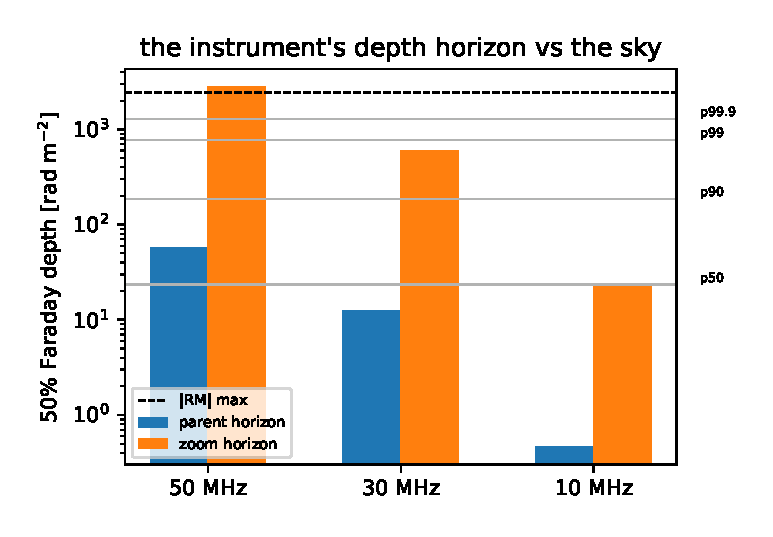
\includegraphics[width=0.62\textwidth]{step5_envelope.pdf}
  \caption{Depth horizons against the beam-weighted sky. Horizontal
  lines are the percentiles of Table~\ref{tab:horizon}; dashed is the
  map maximum.}
  \label{fig:envelope}
\end{figure}

\subsection{Where the cut sits relative to the resolution}
\label{sec:cutresolution}

This matters for Section~\ref{sec:detection} and it is
basis-independent. The systematics cut at $\phi \ge \SafeCut$\,\rmu{}
sits \cutResThirty{} amplitude resolution elements from the origin at
30\,MHz, but only \cutResFifty{} at 50\,MHz, where the resolution is
\resAmpFifty\,\rmu{} rather than \resAmpThirty.

So although 50\,MHz has the larger raw SNR (Section~\ref{sec:detection}),
\textbf{30\,MHz is the band where the cut is cleanly executable}: at
50\,MHz the separation between signal and $\phi\approx0$ leakage rests
entirely on window sidelobe control rather than on resolution. That is
a better reason to lead with 30\,MHz than the knee ever was.

\section{The amplitude bracket}
\label{sec:bracket}

The observable is a fractional polarized amplitude referred to
$T_{\rm sky}$. Three levels are computed and only their provenance
makes them usable.

\subsection{Incoherent patches (upper)}

With $N_{\rm patch}$ independent-angle patches in the beam,
\begin{equation}
  A_{\rm upper} = N_{\rm patch}^{-1/2},
  \qquad N_{\rm patch} = \Omega_{\rm beam}/\theta_c^{2},
  \label{eq:upper}
\end{equation}
with $\Omega_{\rm beam}$ the participation-ratio solid angle of the
weight and $\theta_c$ from the RM structure function $D(\theta)$ via
\begin{equation}
  2\lambda^{4} D(\theta_c) = 1,
  \label{eq:thetac}
\end{equation}
the separation at which the RMS differential rotation of the
polarization angle, $2\Delta\phi\lamsq$, reaches $\sqrt2$ radians.
Section~\ref{sec:cannot} shows this map cannot resolve
Equation~\eqref{eq:thetac}, which is why $A_{\rm upper}$ appears in no
verdict below.

\subsection{The two power-law floors}

Both come from depolarisation \emph{within} the emitting volume, and
the mixed-versus-external distinction is the whole question.

\paragraph{Uniform slab.} For emission spread uniformly through a
rotating column --- the $k=0$ geometry of
Section~\ref{sec:pushforward} ---
\begin{equation}
  \frac{P}{P_0} = \left|\int_0^1 e^{2if\phi_{\rm col}\lamsq}\mathrm df\right|
  = \left|\frac{\sin(\phi_{\rm col}\lamsq)}{\phi_{\rm col}\lamsq}\right|
  \;\xrightarrow[\phi_{\rm col}\lamsq \gg 1]{}\;
  \frac{1}{\phi_{\rm col}\lamsq},
  \qquad
  A_{\rm slab} = \frac{1}{|\phi_{\rm med}|\lamsq}.
  \label{eq:slab}
\end{equation}
Note the factor: under $e^{+2i\phi\lamsq}$ the modulus is
$|\sin(\phi\lamsq)/(\phi\lamsq)|$, \emph{not}
$\operatorname{sinc}(2\phi\lamsq)$.

\paragraph{Internal dispersion.} For a mixed medium with turbulent
dispersion $\sigma$ co-spatial with the emission
\citep{burn1966,sokoloff1998},
\begin{equation}
  \frac{P}{P_0} = \frac{1-e^{-2\sigma^{2}\lambda^{4}}}{2\sigma^{2}\lambda^{4}}
  \;\xrightarrow[2\sigma^2\lambda^4 \gg 1]{}\;
  \frac{1}{2\sigma^{2}\lambda^{4}},
  \qquad
  A_{\rm disp} = \frac{1}{2\sigma_{\rm eff}^{2}\lambda^{4}}.
  \label{eq:disp}
\end{equation}

\paragraph{Why both are power laws, and why it decides everything.}
For an \emph{external} screen the same dispersion gives Burn's
exponential $P/P_0 = e^{-2\sigma^2\lambda^4}$. At these wavelengths
that is not a small number, it is zero: at 30\,MHz the exponent is
$\approx1.9\times10^{6}$. \textbf{A mixed geometry converts exponential
suppression into a power law, and that conversion is the difference
between a detectable signal and no signal at all.} Which of
Equations~\eqref{eq:slab} and~\eqref{eq:disp} the interstellar medium
sets is not determined here, and it is the single unknown the science
case turns on.

Neither floor contains $\theta_c$; a clamped coherence angle
contaminates $A_{\rm upper}$ alone.

\begin{table}[htbp]
  \centering
  \caption{The amplitude bracket, as fractional polarized amplitude
  referred to $T_{\rm sky}$.}
  \label{tab:bracket}
  \begin{tabular}{lccc}
    \toprule
    Level & 30\,MHz & 50\,MHz & 10\,MHz \\
    \midrule
    \BracketRows
    \midrule
    \multicolumn{4}{l}{\emph{$A_{\rm upper}$ is not computable from
    this map (\S\ref{sec:cannot}); it enters no verdict.}}\\
    \bottomrule
  \end{tabular}
\end{table}

\section{Noise and the matched filter}
\label{sec:noise}

Per bin of width $\Delta\nu$ and integration $\Delta t$,
$\sigma = T_{\rm sys}/\sqrt{\Delta\nu\Delta t}$. The zoom bins are not
independent: their equivalent noise bandwidth is $563$\,Hz on
$390.625$\,Hz spacing, a $1.44\times$ overlap, so with $G = W^{\!\top}W$
for the column-normalised fine-to-bin weight matrix,
\begin{equation}
  N_{ij} = \sigma^{2}\,\frac{G_{ij}}{\sqrt{G_{ii}G_{jj}}},
  \label{eq:noisecov}
\end{equation}
unit-diagonal by construction with a measured nearest-neighbour
correlation of $0.15$.

There is no waveform to match, and that is what shapes the statistic.
The intrinsic polarization angles are unknown, so $P(\lamsq)$ carries a
random phase and a classical matched filter --- correlate the data
against a known template --- has nothing to correlate against. What
\emph{is} predictable is the second moment: a signal of amplitude $A$
contributes $A^2S$ to the channel covariance, so the data covariance is
$C(A) = N + A^2 S$ and the question becomes whether the data carries
extra covariance of a known shape. The optimal test for that is
quadratic rather than linear,
\begin{equation}
  q \;=\; d^{\dagger} N^{-1} S N^{-1} d ,
  \label{eq:score}
\end{equation}
whose mean shifts by $A^2\operatorname{tr}[(N^{-1}S)^2]$ against a
noise-only scatter of $\operatorname{tr}[(N^{-1}S)^2]^{1/2}$. Coadding
$M$ independent LST samples and $n$ coherent nights gives
$\mathrm{SNR} = nA^2\sqrt{M\operatorname{tr}[(N^{-1}S)^2]}$, which
inverts to Equation~\eqref{eq:mf}. Note $A \propto
\operatorname{tr}^{-1/4}$: the statistic is quadratic in $A$ and the
signal-to-noise quadratic again, so even a factor of two in the Fisher
information is only $2^{1/4}$ in amplitude.

Whitening is not cosmetic. $N^{-1}$ on both sides upweights the channel
combinations where $S$'s structure differs most from the noise's, and
of the $192$ zoom channels only \nEffModes{} are effectively
independent by the participation ratio of the eigenvalues of
$N^{-1}S$. Replacing $N$ by its diagonal degrades the threshold by
$\diagPenalty$.

The signal is a Gaussian field of known normalised shape $\hat H$ and
unknown amplitude $A$, with the frequency covariance
$S_{ij}$ of Equation~\eqref{eq:sij} --- the depth transform read on the
channel separation --- normalised so $\sum_b \hat H_b = 1$ and hence
$\mathrm{diag}(S) = 1$. For $M$ LST samples and $n$ coherent nights
\begin{equation}
  A_{5\sigma} = \sqrt{\frac{5}{n\sqrt{M\operatorname{tr}[(N^{-1}S)^2]}}}.
  \label{eq:mf}
\end{equation}
Equation~\eqref{eq:mf} carries Equation~\eqref{eq:noisecov} rather than
assuming independent modes; replacing $N$ by its diagonal and holding
everything else fixed degrades the threshold by a measured
$\mathbf{\diagPenalty}$. That ratio, and not any comparison to a closed
form, is the cost of the overlap.

A closed form on \emph{different} assumptions --- noise per coherence
cell, independent modes --- is carried as a sanity check. It agrees to
$2\%$ at 30\,MHz and diverges at the other bands (the matched filter is
$16\%$ worse at 50\,MHz and $46\%$ better at 10\,MHz), because a fixed
coherence bandwidth is a poor description of the real signal covariance
there. It is a check, not a bound.

Figure~\ref{fig:sensitivity} gives the threshold curve against
lunations, with the bracket overlaid.

\begin{figure}[htbp]
  \centering
  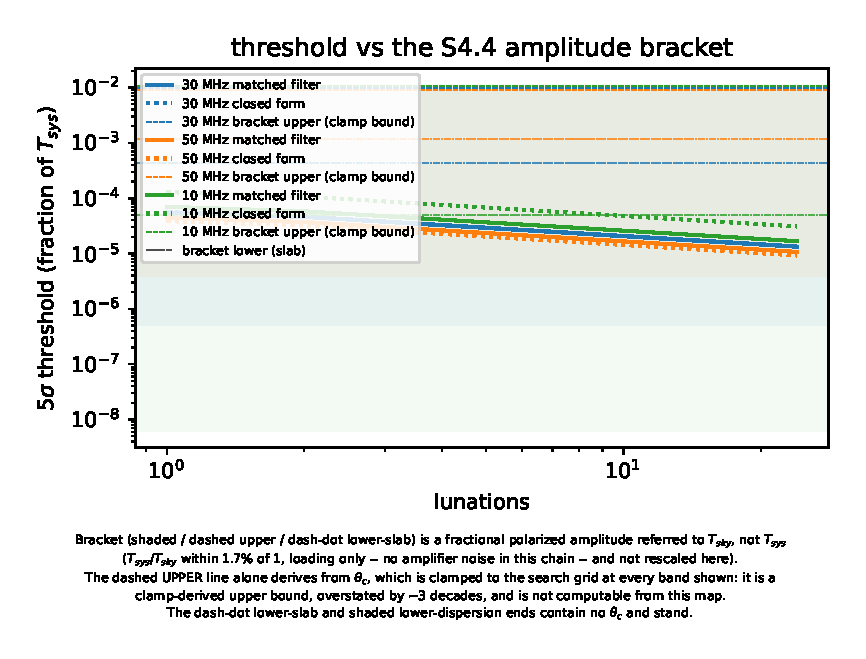
\includegraphics[width=0.78\textwidth]{step5_sensitivity.pdf}
  \caption{The $5\sigma$ threshold against lunations for the
  \emph{full} template, with the closed form dotted and the bracket
  shaded. Section~\ref{sec:detection} is the version with the
  systematics cut applied; this figure is the uncut reference.}
  \label{fig:sensitivity}
\end{figure}

\section{Detection SNR against the systematics cut}
\label{sec:detection}

\subsection{The statistic, and why there is a cut}

Instrumental $I\!\to\!Q,U$ leakage passes through a frozen beam and is
therefore spectrally smooth, which puts it at $\phi\approx0$ --- and at
$\tau\approx0$. A detection statistic that integrates all depths is
degenerate with it. The cut is what breaks the degeneracy, and its
position comes from the window budget: against a $\phi\approx0$
foreground at $|P|/I = 0.15$ through a four-term Blackman--Harris
window \citep{harris1978}, leakage into depth is $3.7\times10^{-6}$ at
the first sidelobe ($\phi\approx10.8$) and $\le10^{-6}$ beyond
$\phi = \SafeCut$. That is the cut used throughout.

For a cut retaining power fraction $f$, the detectable quantity is
$A_{\rm bracket}\sqrt f$ --- $\sqrt f$ and not $f$, because $f$ is a
fraction of \emph{power} and the bracket is an \emph{amplitude} --- and
the threshold is Equation~\eqref{eq:mf} computed on the
\textbf{truncated} template. That last point is not a detail: a
statistic looking only above the cut has only the truncated shape to
match against, and its threshold is $28$--$35\%$ higher than the full
template's. An earlier version of this document compared a truncated
signal against a full-template threshold.

\subsection{The result}

\begin{table}[htbp]
  \centering
  \caption{Detection ratio $A_{\rm bracket}\sqrt f / A_{5\sigma}$ at
  \Lunations{} lunations. Above 1 is a $5\sigma$ detection. ``keeps''
  is the retained template power fraction.}
  \label{tab:detection}
  \begin{tabular}{lc cc cc cc}
    \toprule
    & & \multicolumn{2}{c}{30\,MHz} & \multicolumn{2}{c}{50\,MHz}
      & \multicolumn{2}{c}{10\,MHz} \\
    \cmidrule(lr){3-4}\cmidrule(lr){5-6}\cmidrule(lr){7-8}
    cut $\phi$ & keeps & slab & disp & slab & disp & slab & disp \\
    \midrule
    \DetectionRows
    \bottomrule
  \end{tabular}
\end{table}

\begin{figure}[htbp]
  \centering
  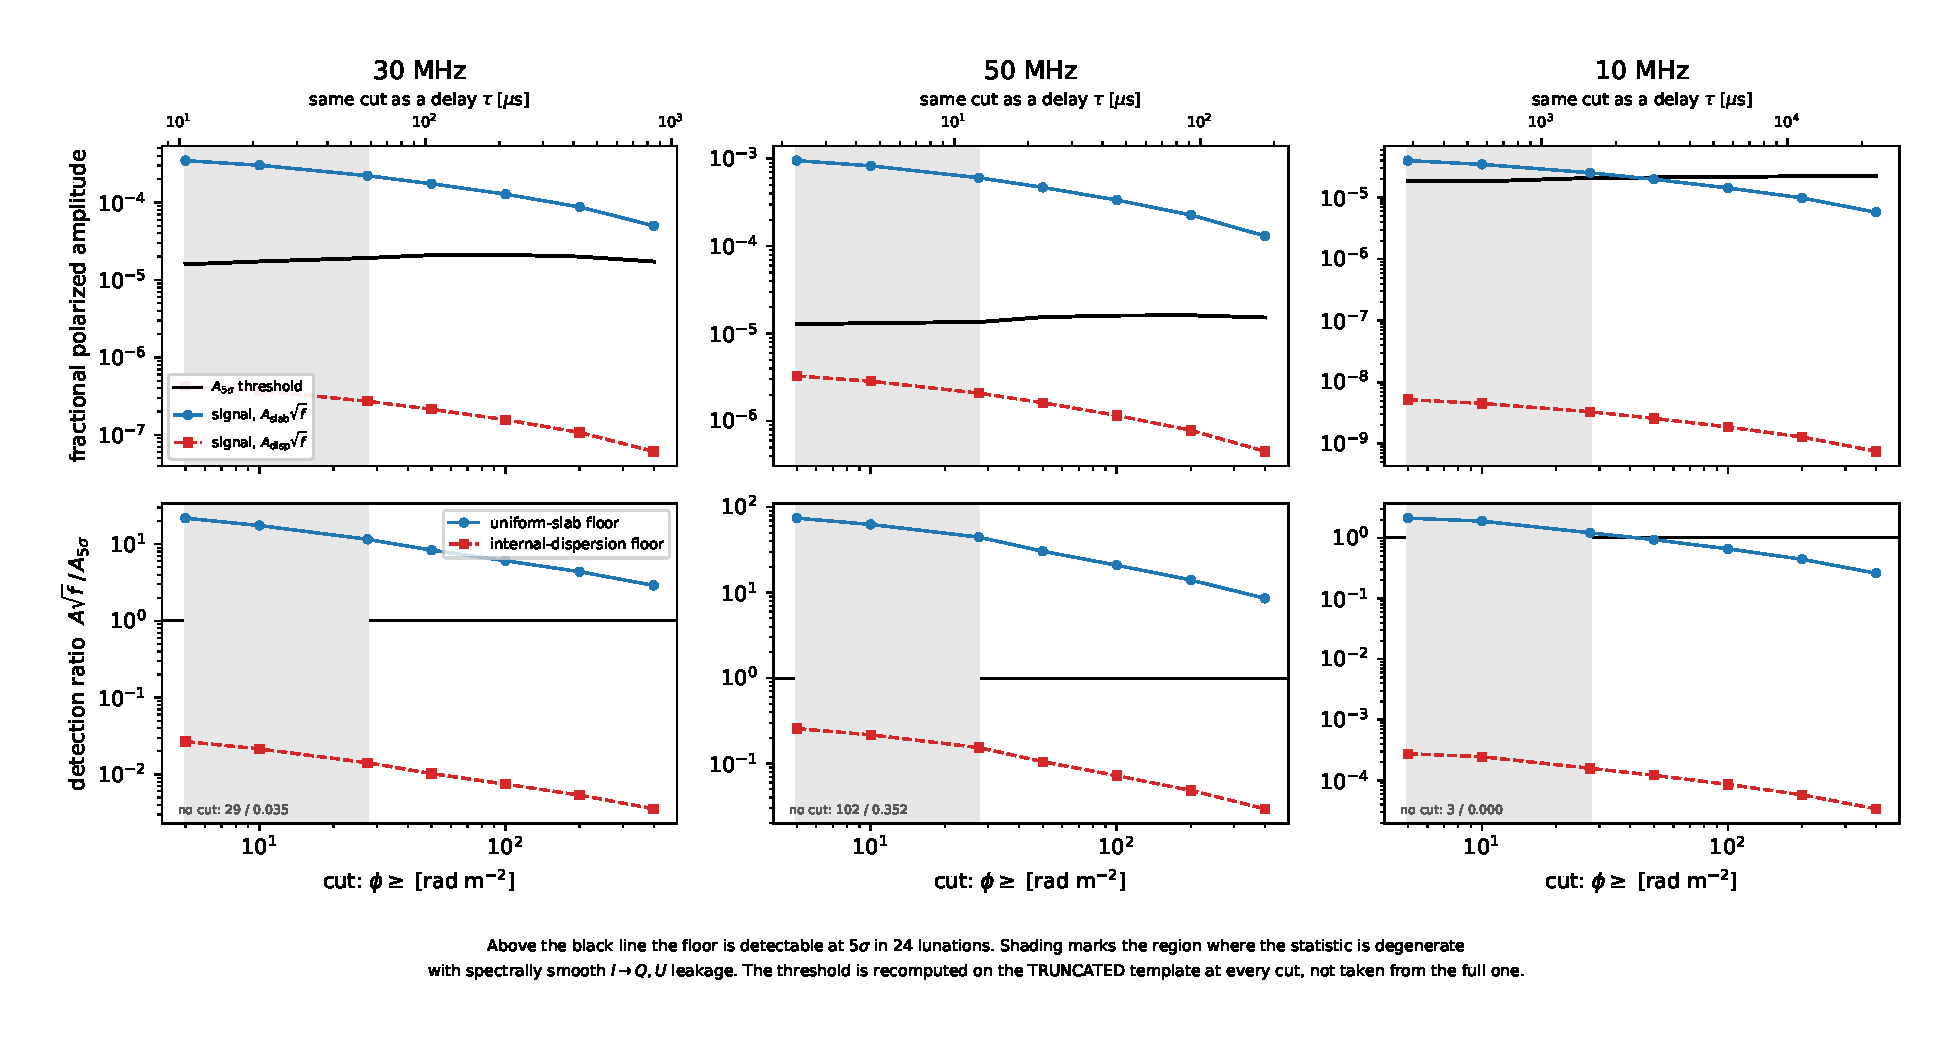
\includegraphics[width=\textwidth]{step5_detection.pdf}
  \caption{Detection ratio against the systematics cut. The top axis of
  each panel is the same cut expressed as a delay
  (Equation~\eqref{eq:taufd}), so the figure is readable in either
  basis. Shading marks the region degenerate with smooth leakage.}
  \label{fig:detection}
\end{figure}

At the systematics-safe cut, retaining $\keepFracThirty$\% of the
template power:

\begin{itemize}
  \item \textbf{At the uniform-slab floor the signal is detectable} at
    30 and 50\,MHz --- $\detSafeSlabThirty\times$ threshold and
    $\detSafeSlabFifty\times$. At 10\,MHz it is
    $\detSafeSlabTen\times$, which is above threshold but marginal:
    it does not survive the coherent limit of
    Section~\ref{sec:tilt}, and 10\,MHz is also the band whose delay
    basis aliases (Appendix~\ref{sec:bases}).
  \item \textbf{At the internal-dispersion floor it is not}, at any
    band: $\detSafeDispThirty$ at 30\,MHz, $\detSafeDispFifty$ at
    50\,MHz, $\detSafeDispTen$ at 10\,MHz.
  \item \textbf{The cut is cheap.} It costs a factor
    $\cutCostThirty$ in sensitivity at 30\,MHz and
    $\cutCostFifty$ at 50\,MHz --- the threshold rises only modestly
    because the truncated template still spans most of the axis.
\end{itemize}

\subsection{What does not decide it}

\paragraph{Not the basis.} Every row of Table~\ref{tab:detection} is a
cut in delay as much as in depth (Appendix~\ref{sec:bases}); the safe cut
is $\tauSafeThirty\,\mu$s at 30\,MHz and $\tauSafeFifty\,\mu$s at
50\,MHz.

\paragraph{Not $\theta_c$.} Both floors are $\theta_c$-free by
Equations~\eqref{eq:slab} and~\eqref{eq:disp}.

\paragraph{Not integration time, though less decisively than once
claimed.} With $n_{\rm lst}$ saturated by \Lunations{} lunations the
threshold falls as $n^{-1/2}$, so closing a gap costs its square. At
50\,MHz the dispersion-floor gap after the cut is
$\dispGapSafeFifty\times$, an observing-time factor of
$\dispTimeSafeFifty$ --- long against a two-year mission but not
absurd. At 30\,MHz it is $\dispGapSafeThirty\times$, a factor
$\dispTimeSafeThirty$, which is out of reach.

\paragraph{Not the instrument arm.} See Section~\ref{sec:robust}.

\section{Localisation: the tail gate}
\label{sec:tail}

Localisation needs power above the bulk of the sky's depth
distribution. Defining the tail fraction as template power above the
fixed beam-weighted p99 threshold, resolved over sidereal time
(Figure~\ref{fig:knee}), it peaks sharply at Galactic Centre transit
and falls to $\sim10^{-6}$ away from it.

Two things have to be held fixed here, and an earlier version of this
gate held neither.

\paragraph{The geometry must match.} The stored per-LST tail fraction
is computed by binning the raw \emph{column} depth $\phi_{\rm col}$
weighted by $|w|^2$ --- that is the $k\to\infty$ distribution, all
emission at the far end. Every other number in this report uses the
fiducial $k=0$ slab, whose pushforward
(Equation~\eqref{eq:pushforward}) spreads mass down toward $\phi = 0$
and leaves $4.4$--$4.9\times$ less tail. Mixing a $k\to\infty$ tail
fraction with a $k=0$ bracket inflates the gate by about that factor.
The numbers below are the fiducial geometry throughout.

\paragraph{The threshold must match the statistic.} A statistic looking
only above the cut has only the truncated shape to match against, so
its threshold is the one computed on the truncated transit-time
template, not on the full one (Section~\ref{sec:detection}).

Done consistently on both counts, the ratios at the uniform-slab floor
are $\tailSlabThirty$ at 30\,MHz, $\tailSlabFifty$ at 50\,MHz and
$\tailSlabTen$ at 10\,MHz; the two-port arm gives
$\tailSlabTwoPortThirty$, $\tailSlabTwoPortFifty$ and
$\tailSlabTwoPortTen$, so the calls do not depend on which arm weights
the sky.

So localisation is \textbf{marginal} at 30\,MHz even at the slab floor,
plausible only at 50\,MHz, and out of reach at the dispersion floor
everywhere --- which is why this report treats detection as the
deliverable and localisation as the stretch goal, and not the other way
round. Compare the detection ratios of Table~\ref{tab:detection}, which
are an order of magnitude larger at the same cut.

\begin{figure}[htbp]
  \centering
  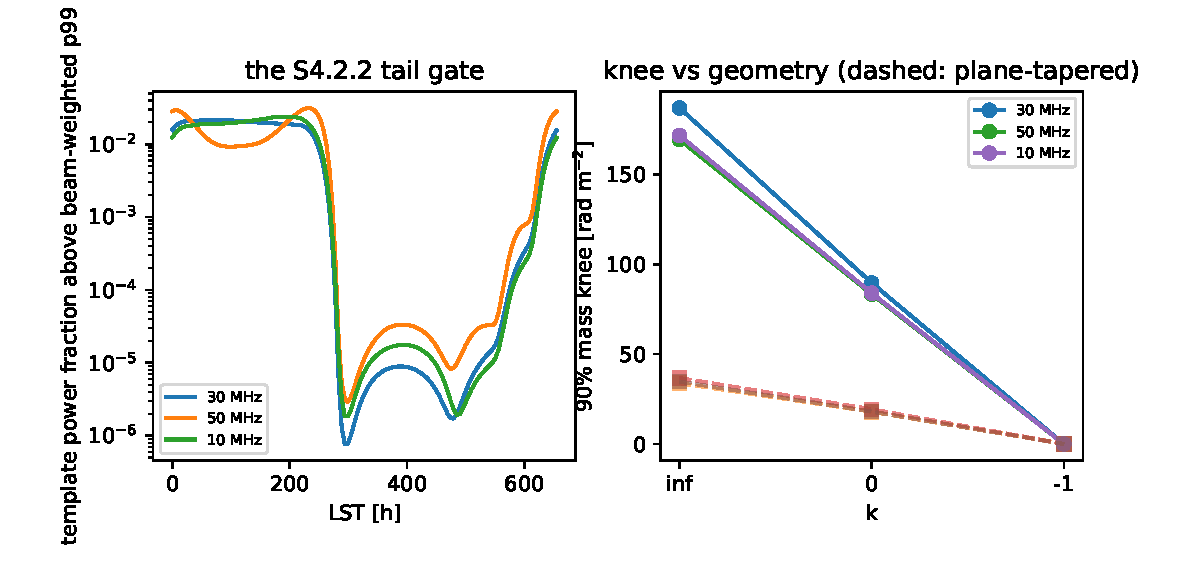
\includegraphics[width=\textwidth]{step5_knee_tail_lst.pdf}
  \caption{Left: tail fraction over sidereal time, peaking at Galactic
  Centre transit. Right: the 90\%-mass knee per band against the
  emissivity geometry, plane-tapered version dashed.}
  \label{fig:knee}
\end{figure}

\section{What this map cannot decide}
\label{sec:cannot}

\subsection{The bracket's upper end}
\label{sec:clamp}

$\theta_c$ is the separation beyond which the sky's polarization angle
no longer stays coherent after rotation. With the RM structure function
$D(\theta) = \langle({\rm RM}(\hat n_1)-{\rm RM}(\hat n_2))^2\rangle$,
two sightlines separated by $\theta$ differ in angle by
$2\sqrt{D(\theta)}\,\lamsq$ in the RMS; setting that to $\sqrt2$
radians gives Equation~\eqref{eq:thetac}. It is a \emph{two-point}
statistic, which is why it cannot be recovered from the template at all
--- $F$ is a one-point object (Section~\ref{sec:depthdist}) and
\code{structure\_function} has to return to the map itself.

Equation~\eqref{eq:thetac} is solved by inverting a Monte-Carlo
$D(\theta)$ on a grid spanning $0.2^\circ$--$30^\circ$. At every band
and in both arms the solution \textbf{clamps at the grid's lower edge}
(\thetaCDeg$^\circ$; all clamped: \thetaCAllClamped).

The clamp \emph{overstates}: a target below $D(\theta_{\min})$ means the
root lies below the grid, so returning $\theta_{\min}$ returns
something larger, and $A_{\rm upper}\propto\theta_c$ inherits it.
Measured on the script's own grid, $D(0.2^\circ) = 96.2\,(\rmu)^2$
against targets $5.01\times10^{-5}$, $3.87\times10^{-4}$ and
$6.19\times10^{-7}$ --- a root $1385\times$, $499\times$ and
$12\,465\times$ below the grid edge under $D\propto\theta^2$.

\textbf{Widening the grid cannot fix it.} Extrapolation puts the root
at $0.52''$, $1.44''$ and $0.058''$, two and a half to nearly four
decades below the $412''$ pixel scale of the Faraday map itself. The
internal evidence that the extrapolation is unquotable is that it
inverts the bracket: at 30\,MHz it gives $7.1\times10^{-6}$, below
$A_{\rm slab} = \bracketSlabThirty$.

\subsection{The coherent limit of the template shape}
\label{sec:tilt}

Equation~\eqref{eq:deposit} adds contributions to a depth bin in
\emph{power}. The opposite limit adds them in amplitude, so a bin fed
by $N$ coherence patches gains $N^2$ where the incoherent sum gains
$N$. Were $N$ the same in every bin this would be one global factor and
would vanish under normalisation; it does not vanish, because $N$ falls
steeply with depth --- low depths draw on the whole high-latitude sky,
high depths only on the narrow Galactic plane. The coherent limit is
therefore a statement about the template's \emph{shape}, and a large
one: at 30\,MHz it would cut the retained fraction to \tiltFracThirty,
move the 90\%-mass knee to \tiltKneeThirty\,\rmu, and cost a factor
\tiltFactorThirty{} in detection ratio at the slab floor, taking
\detSafeSlabThirty{} to \tiltAppliedThirty. At 10\,MHz the factor is
\tiltFactorTen, taking \detSafeSlabTen{} to \tiltAppliedTen{} ---
below threshold.

It is quoted as a \emph{factor} deliberately. The tilt is a folded
shape statement with no signed twin stored, so its own threshold is
built on the folded template, whereas
Table~\ref{tab:detection} is built on the signed one
(Section~\ref{sec:roadmap}). Dividing two folded numbers cancels that
difference; comparing a folded tilt against a signed baseline would
conflate the coherence question with the basis convention and
understate the tilt by about a fifth.

\textbf{It is not computable here, for exactly the reason of
Section~\ref{sec:clamp}.} The patch count needs $\theta_c$, which
clamps (\tiltThetaCDeg$^\circ$; all clamped: \tiltThetaCClamped) with
its true root below the grid and below the nside-512 pixel scale of
\pixelScaleDeg$^\circ$, so the map cannot resolve the patches the
construct is built from. This is the shape-space sibling of
$A_{\rm upper}$, it has the identical defect, and it is treated the
same way: quantified here, and entering no verdict. It is deliberately
not drawn in Figure~\ref{fig:family}, where a peer curve would read as
a live alternative.

Section~\ref{sec:identity} does not settle this. That identity holds
even for a maximally coherent sky ($\alpha_n \equiv 0$ passes at
$0.889$), because at nside 512 neighbouring pixels sit hundreds of
carrier turns apart and their cross terms cancel by oscillation rather
than by phase randomness. It therefore validates
Equation~\eqref{eq:deposit} at and above the pixel scale and says
nothing about coherent structure below it --- which is the regime
$\theta_c$ parameterises.

\subsection{Turbulence enters the amplitude but not the shape}
\label{sec:sigmashape}

Section~\ref{sec:bracket}'s dispersion floor asserts turbulent Faraday
depth of dispersion $\sigma_{\rm eff}$ co-spatial with the emission.
The template does not contain it. $F$ is built from the map's resolved
column depths and the $f^k$ geometry
(Equation~\eqref{eq:deposit}); $\sigma_{\rm eff}$ enters only
Equation~\eqref{eq:disp}, as an amplitude.

That is inconsistent. If the turbulence is there it should broaden $F$
as well, and broadening moves mass across the low-depth cut: convolving
the fiducial template with a Gaussian of the fiducial
$\sigma_{\rm eff} = \sigmaEff$\,\rmu{} raises the detection ratio by
$\sigmaBroadenOne\%$, and by twice that dispersion, by
$\sigmaBroadenTwo\%$. The effect is favourable and modest at
the fiducial value, but the direction is not the point --- the same
physical assumption is being used in one place and ignored in another.

Two things bound how much this can matter. The correct kernel is not a
uniform convolution: for co-spatial turbulence the scatter accumulates
along the path, so it should grow with $f$ rather than apply equally to
every depth. And $\sigma_{\rm eff}$ is an assumed input, not a measured
one --- unlike $k$, which Section~\ref{sec:kscan} scans, it is a single
default value carrying the factor \floorRatioThirty{} between the two
floors. \textbf{The least-scrutinised input in this report is the one
the verdict is most sensitive to.}

\subsection{Sky domination at 50\,MHz}

$T_{\rm sys}/T_{\rm sky} = \tsysThirty / \tsysFifty / \tsysTen$ at
$30/50/10$\,MHz. Read it as $1 + T_{\rm loading}/T_{\rm sky}$ and
nothing more: the modelled chain carries \textbf{no amplifier noise},
so the term this check exists to bound --- receiver noise through a
short, mismatched dipole on regolith at 50\,MHz --- is set to zero, and
$T_{\rm sky}$ is an all-sky Stokes $I$ mean rather than a beam-weighted
antenna temperature. It is a genuine \emph{lower bound}. What it does
establish is that loading is a $\le\tsysMaxPct$\% correction, so the
reference-temperature mismatch in Figure~\ref{fig:sensitivity} is
negligible. \textbf{Sky domination at 50\,MHz remains open.}

\subsection{Two limits already stated}

The acceptance gates do not test the incoherent-limit identity, and the
identity does not demonstrate that the sky is incoherent
(Section~\ref{sec:identity}).

\section{Reconciliation with the earlier analysis}
\label{sec:reconcile}

\begin{center}
\begin{tabular}{lll}
\toprule
Earlier section & Status & Where it now lives \\
\midrule
Step 0, calibrated polarimeter & stands & unchanged \\
Step 1, single polarized source & stands & regenerated, $\le0.6\%$ moves \\
Step 3, 10 and 50\,MHz bands & stands & unchanged \\
Perfect-depolarisation ($I$-only) limit & stands & unchanged \\
\midrule
Step 2, the real sky at 30\,MHz & \textbf{refuted} & \S\ref{sec:randomwalk}--\ref{sec:depthdist} \\
Step 4, delay-space signature & \textbf{superseded}
  & App.~\ref{sec:bases}, \S\ref{sec:detection} \\
\bottomrule
\end{tabular}
\end{center}

The distinction in the last two rows is deliberate. Step 2 is
\emph{refuted}: its diffuse signature was a pixelisation artifact, and
the quantity $|\Delta P|/I \sim 1.7\times10^{-4}$ does not appear here
in any form. Step 4 is \emph{superseded} but not wrong about its
basis: Appendix~\ref{sec:bases} finds the delay axis it used to be
sound at 30 and 50\,MHz, and its own $\tau_{\rm FD}$ scale --- 5\,ms at
30\,MHz and 1.1\,ms at 50\,MHz for $\phi_{\max}\approx2400$ ---
reproduces Equation~\eqref{eq:taufd} exactly. What it inherited from
Step 2 was the shot-noise amplitude, not the transform.

Cite the tag, not a branch, when referring to those results. Nothing
here modifies that document.

\section{Reproducing this}
\label{sec:repro}

No number in this document is typed by hand: all of them live in
\code{generated.tex}, written by \code{scripts/step5\_tables.py}
straight from the \code{.npz} products. That file and the figures are
tracked, so the report builds from a fresh checkout.

\begin{center}
\begin{tabular}{lll}
\toprule
Product & Script & Contains \\
\midrule
\code{step5\_envelope.npz} & \code{step5\_instrument\_envelope.py}
  & Table~\ref{tab:horizon} \\
\code{step5\_template.npz} & \code{step5\_template.py --lst 128}
  & Tables~\ref{tab:bracket},~\ref{tab:robust} \\
\code{step5\_template\_two\_port.npz} & \code{... --arm two-port}
  & arm columns \\
\code{step5\_sensitivity.npz} & \code{step5\_sensitivity.py}
  & Figure~\ref{fig:sensitivity} \\
\code{step5\_detection.npz} & \code{step5\_detection.py}
  & Table~\ref{tab:detection}, \S\ref{sec:tail} \\
figures & \code{step5\_plots.py} & all \\
numbers & \code{step5\_tables.py} & \code{generated.tex} \\
\bottomrule
\end{tabular}
\end{center}

Table~\ref{tab:rmsf} is computed live in about two seconds and needs no
data products. A companion notebook,
\code{notebooks/faraday\_depth\_template.ipynb}, is committed executed.

\subsection{Which test pins which claim}

\begin{center}
\footnotesize
\begin{tabular}{ll}
\toprule
Claim & Test \\
\midrule
Shape stable under refinement
  & \code{test\_gate1\_shape\_invariance\_under\_refinement} \\
Shape stable under null rotation
  & \code{test\_gate2\_shape\_invariance\_under\_null\_rotation} \\
The identity, Eq.~\eqref{eq:identity}
  & \code{test\_depth\_power\_equals\_the\_weighted\_depth\_distribution} \\
Converged control through the NUFFT
  & \code{test\_converged\_regime\_points\_match\_direct\_sum} \\
Depth horizons, Table~\ref{tab:horizon}
  & \code{test\_depth\_horizon\_pins\_the\_s46\_table} \\
Resolution and convention, Table~\ref{tab:rmsf}
  & \code{test\_boxcar\_rmsf\_widths} \\
The chirp, \S\ref{sec:bases}
  & \code{test\_nufft\_beats\_fft\_on\_a\_single\_depth} \\
Window budget, \S\ref{sec:detection}
  & \code{test\_foreground\_sidelobe\_budget} \\
$\theta_c$ clamps below the grid, \S\ref{sec:clamp}
  & \code{test\_coherence\_angle\_clamps\_below\_the\_sampled\_range} \\
Bracket closed forms, Eqs.~\eqref{eq:slab},~\eqref{eq:disp}
  & \code{test\_amplitude\_bracket\_closed\_forms} \\
Overlap degradation $\diagPenalty\times$
  & \code{test\_overlap\_correlation\_degrades\_the\_threshold} \\
Matched filter, Eq.~\eqref{eq:mf}
  & \code{test\_matched\_filter\_monte\_carlo} \\
\bottomrule
\end{tabular}
\end{center}

\subsection{Building}

\begin{verbatim}
    uv run python scripts/step5_detection.py     # the detection npz
    uv run python scripts/step5_tables.py        # generated.tex
    uv run python scripts/step5_plots.py         # the figures
    cd report/faraday_depth_template && make
\end{verbatim}

\appendix

\section{Faraday depth and delay are the same measurement}
\label{sec:bases}

\textbf{This appendix settles a question the present analysis does not
face.} Nothing in Sections~\ref{sec:depthdist}--\ref{sec:detection}
transforms data into either basis: the template lives in depth, the
statistic lives in the channel covariance
(Equation~\eqref{eq:sij}), and no delay spectrum and no depth spectrum
is ever formed from a measurement. Delay appears in the main text only
as an alternative label on the cut axis of
Figure~\ref{fig:detection}. The basis question matters because the
superseded Step 4 worked in delay, and Section~\ref{sec:reconcile}
has to say whether that was sound. It was, at 30 and 50\,MHz.

Faraday depth $\phi$ is the Fourier conjugate of $\lamsq$. Delay $\tau$
is the Fourier conjugate of $\nu$. They are not the same axis, and this
report keeps them distinct --- but for detection they carry the same
information, and it is worth saying why, because the earlier analysis
worked in $\tau$ and the argument against it has been overstated.

\subsection{The mapping}

The phase of a single depth is $\Theta(\nu) = 2\phi c^2/\nu^2$, so
against an FFT kernel $e^{-2\pi i\nu\tau}$ its local delay is
\begin{equation}
  \tau_{\rm FD}(\phi,\nu)
  = -\frac{1}{2\pi}\frac{\mathrm d\Theta}{\mathrm d\nu}
  = \frac{2\phi c^2}{\pi\nu^3}.
  \label{eq:taufd}
\end{equation}
Equation~\eqref{eq:taufd} is \emph{monotonic} in $\phi$, so a cut at
$\phi \ge \phi_{\min}$ is exactly a cut at
$\tau \ge \tau_{\rm FD}(\phi_{\min})$ and retains identically the same
power. Every detection number in Section~\ref{sec:detection} is
therefore a statement about the measurement, not about the basis. (It
is also $\nu$-dependent, which is the one thing that does not transfer:
the same sky sits at different delays in different bands, so 30 and
50\,MHz cannot be combined on one delay axis.)

\subsection{The chirp is negligible against a broad template}

Because $\tau_{\rm FD} \propto \nu^{-3}$, a single depth drifts in
delay across the band --- the chirp. The relevant question is not
whether the chirp exists but whether it is large compared with the
structure being measured, and it is not:

\begin{center}
\begin{tabular}{lccccc}
\toprule
Band & extent & chirp smear & \textbf{smear/extent}
  & aliasing wall & aliased/kept \\
 & \multicolumn{2}{c}{(delay resolution elements)} &
  & (\rmu) & signal \\
\midrule
\BasisRows
\bottomrule
\end{tabular}
\end{center}

\textbf{Our signal is not a peak.} It is a broad, monotonically falling
distribution spanning hundreds of resolution elements; smearing it by
1--2\% of its own width changes nothing. The chirp destroys information
only when a \emph{narrow} feature must be resolved --- that is,
localisation. Figure~\ref{fig:chirp} shows the effect on a single
injected depth, which is the case where it matters most.

The one genuine failure is 10\,MHz, and it fails on \emph{aliasing},
not the chirp: $30\%$ of its template power sits beyond the
delay-Nyquist wall and folds back onto the signal. At 30 and 50\,MHz
that contamination is \aliasPctThirty\% and \aliasPctFifty\%. Notably
the aliasing wall (\aliasWallThirty{} and \aliasWallFifty\,\rmu) and
the instrument's own depth horizon (\zoomHorThirty{} and
\zoomHorFifty, Section~\ref{sec:horizon}) coincide to $0.1\%$ at all
three bands --- measured, and not something this work explains --- so
aliasing never binds where the bin response has not already
attenuated.

\begin{figure}[htbp]
  \centering
  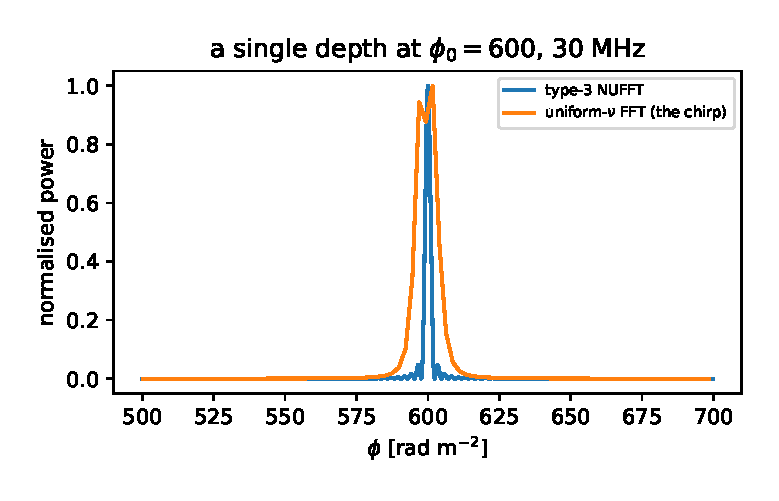
\includegraphics[width=0.62\textwidth]{step5_chirp_coherence.pdf}
  \caption{A single Faraday depth at $\phi_0 = 600$\,\rmu, 30\,MHz,
  transformed on the true \lamsq{} nodes and by an FFT on a uniform
  $\nu$ grid. This is the worst case for the delay basis --- one narrow
  feature. Against the broad template of Figure~\ref{fig:family} the
  same chirp is 2\% of the extent.}
  \label{fig:chirp}
\end{figure}

\subsection{Which basis to use}

For \textbf{detection}, either. The matched filter of
Section~\ref{sec:noise} builds its signal covariance from the true
\lamsq{} of the bins, so it carries the exact chirped phases and is the
optimal statistic regardless of how the result is plotted.

For everything else, $\phi$: it is in \rmu{} and comparable with the RM
literature, the deconvolution kernel is shift-invariant in $\phi$ but
$\phi$-dependent in $\tau$, and bands can be combined. This work
computes in $\phi$ for those reasons and not because the delay basis
fails.

\section*{Acknowledgements}

This work uses the Galactic Faraday rotation sky of
\citet{hutschenreuter2022}, the destriped 408\,MHz map of
\citet{remazeilles2015}, the nine-year WMAP polarization maps of
\citet{bennett2013}, the HEALPix pixelisation \citep{gorski2005}, and
the FINUFFT library \citep{barnett2019}.

\begin{thebibliography}{99}

\bibitem[Barnett et al.(2019)]{barnett2019}
Barnett, A.~H., Magland, J., \& af Klinteberg, L. 2019,
\emph{A Parallel Nonuniform Fast Fourier Transform Library Based on an
``Exponential of Semicircle'' Kernel},
SIAM Journal on Scientific Computing, 41, C479

\bibitem[Bennett et al.(2013)]{bennett2013}
Bennett, C.~L., Larson, D., Weiland, J.~L., et al. 2013,
\emph{Nine-year Wilkinson Microwave Anisotropy Probe (WMAP)
Observations: Final Maps and Results},
ApJS, 208, 20

\bibitem[Brentjens \& de Bruyn(2005)]{brentjens2005}
Brentjens, M.~A., \& de Bruyn, A.~G. 2005,
\emph{Faraday rotation measure synthesis},
A\&A, 441, 1217

\bibitem[Burn(1966)]{burn1966}
Burn, B.~J. 1966,
\emph{On the depolarization of discrete radio sources by Faraday
dispersion},
MNRAS, 133, 67

\bibitem[G\'orski et al.(2005)]{gorski2005}
G\'orski, K.~M., Hivon, E., Banday, A.~J., et al. 2005,
\emph{HEALPix: A Framework for High-Resolution Discretization and Fast
Analysis of Data Distributed on the Sphere},
ApJ, 622, 759

\bibitem[Harris(1978)]{harris1978}
Harris, F.~J. 1978,
\emph{On the use of windows for harmonic analysis with the discrete
Fourier transform},
Proceedings of the IEEE, 66, 51

\bibitem[Hutschenreuter et al.(2022)]{hutschenreuter2022}
Hutschenreuter, S., Anderson, C.~S., Betti, S., et al. 2022,
\emph{The Galactic Faraday rotation sky 2020},
A\&A, 657, A43

\bibitem[Remazeilles et al.(2015)]{remazeilles2015}
Remazeilles, M., Dickinson, C., Banday, A.~J., Bigot-Sazy, M.-A., \&
Ghosh, T. 2015,
\emph{An improved source-subtracted and destriped 408-MHz all-sky map},
MNRAS, 451, 4311

\bibitem[Sokoloff et al.(1998)]{sokoloff1998}
Sokoloff, D.~D., Bykov, A.~A., Shukurov, A., et al. 1998,
\emph{Depolarization and Faraday effects in galaxies},
MNRAS, 299, 189

\end{thebibliography}

\end{document}
